%\documentclass{vldb}
%\documentclass{acm_proc_article-sp}
\documentclass{cidr-2019}
%\documentclass{sig-alternate-05-2015}
%\documentclass[sigconf]{acmart}
%\documentclass[a4,10pt,fleqn]{article}

%%\usepackage{llncsdoc}
%\usepackage{a4wide}
%%\usepackage{amsthm}
%\usepackage{makeidx}
%\usepackage{times}
%\usepackage{epsf}
%\usepackage{graphicx}
%\usepackage{epsfig}
%\usepackage{graphics}
%\usepackage{color}
%\usepackage{url}

%\usepackage[english]{babel} % otherwise, \cite doesn't work with sig-alternate/acm_proc_article-sp
%\usepackage{amsmath} % doesn't play nice with llncs
%%\usepackage{amsthm} % doesn't play nice with llncs
%\usepackage{txfonts}
%%\usepackage{multiFloats}

%\usepackage{pslatex}
%\usepackage[all]{xy}

%% wrap text around (floating) figures
\usepackage{wrapfig}
\setlength{\wrapoverhang}{0mm}


%%%%%%%%%%%%%%%%%%%%%%%%%%%%%%%%%%%%%%%
% pdfcomment for annotations.         %
% Use final to not have them show up. %
%%%%%%%%%%%%%%%%%%%%%%%%%%%%%%%%%%%%%%%
%% \usepackage[final]{pdfcomment}
\usepackage{pdfcomment}

%\newtheorem{theorem}{Theorem}
%\newtheorem{lemma}[theorem]{Lemma}
%\newtheorem{definition}{Definition}

\hyphenation{data-base}

\renewcommand{\textfraction}{0.0}
\renewcommand{\bottomfraction}{1.0}
\renewcommand{\topfraction}{1.0}
\renewcommand{\dbltopfraction}{1.0}
 
\begin{document}

%\title{SQALPEL\\ Discriminative database performance evaluation\\\emph{DEMO PAPER}}
\title{SQALPEL: A database performance platform\\\emph{DEMO PAPER}}
\numberofauthors{4}
\author{
	\alignauthor {M.L. Kersten\\
	\affaddr{CWI}\\
	\affaddr{Amsterdam}
	}%
	\alignauthor{P. Koutsourakis\\
	\affaddr{MonetDB Solutions}\\
	\affaddr{Amsterdam}
	}%
	\alignauthor{S. Manegold\\
	\affaddr{CWI}\\
	\affaddr{Amsterdam}
	}%
	\alignauthor{Y. Zhang \\
	\affaddr{MonetDB Solutions}\\
	\affaddr{Amsterdam}
	}%
}

%}
\maketitle
%\date{}
%\tableofcontents

\begin{abstract}
%the problem
Despite their popularity, database benchmarks only highlight a small
fraction of the capabilities of any given DBMS. They often do not
highlight problematic components encountered in real life database
applications or provide hints for further research and engineering.
%Furthermore, sharing performance knowledge about actual systems
%is hindered by the effort required to conduct sound experiments 
%and the lack of public sharing of results.

%the solution

%The system is modeled after software repositories with a clear separation of concerns, roles, and legal measures.

%how
To alleviate this problem we coined \textit{discriminative performance
  benchmarking} as the way to go. It aids in exploring a larger query search
space to find performance outliers and their underlying cause. The
approach is based on deriving a domain specific language from a sample
complex query to identify and execute a query workload.

%benefits
%We introduce {\sc sqalpel}, a SaaS platform to orchestrate query performance experiments.
The demo illustrates {\sc sqalpel}, a complete platform to collect,
manage and selectively disseminate performance facts, that enables
repeatability studies, and economy of scale by sharing performance
experiences.

\end{abstract}

\maketitle

\section{Introduction}\label{Introduction}
%The workload space for exercising a DBMS is practically infinite. It relies on the database schema, the data distributions, and the (concurrent) query workload. Therefore, systems are evaluated and compared against one-another using standardized benchmarks, research micro-benchmarks or using proprietary proof-of-concept projects.


%standard benchmarks
Standard benchmarks have long been a focal point in business to aid
customers to make an informed decision about a product's expected
performance. The Transaction Processing Counsel currently supports
several benchmarks ranging from OLTP to IoT. An overview of their
active set is shown in Table~\ref{table:tpc-overview}. Surprisingly,
the number of publicly accessible results remains extremely low. Just
a few vendors go through the rigorous process to obtain results for
publication.
%Furthermore, the number of related technical publications on their website is diminishing.\footnote{http://www.tpc.org/information/other/techarticles.asp}

%In many cases, however, only a small fraction of the benchmark is used to highlight progress.
%Partly because implementation of all functionality requires is an effort
%way beyond the resources of a single PhD candidate.
%Moreover, setting up a comparative benchmark for illustrative purposes with the rigor
%as required by TPC is time consuming. 

%To partly alleviate this situation, several projects can be found on Github that will
%install and run TPC benchmarks on open-source database systems.
%Alternatively, new benchmarks frameworks are defined to study a particular functionality.
%5OLTP-bench ~{oltpbench} is the most mature open-source project to embark on such an analysis.
%It is strongly focused on multi-client interaction and combines fifteen different benchmarks
\begin{table}[t]
  %pdfcomment{Panos: Should Action Vector be  Actian Vectorwise?}
  {\small\addtolength{\tabcolsep}{-2.6pt}\begin{tabular*}{\columnwidth}{ | l | l | p{.55\columnwidth} |}
      \hline
      benchmark & reports & systems reported\\
      \hline
      TPC-C & 368 & Oracle, IBM DB2, MS SQLserver, Sybase, SymfoWARE\\
      TPC-DI &0 &\\
      TPC-DS &1 & Intel\\
      TPC-E &77 & MS SQLserver\\
      TPC-H $\leq$ SF-300 & 252 &MS SQLserver, Oracle, EXASOL, Action Vector 5.0, Sybase, IBM DB2, Informix, Teradata, Paraccel\\
      TPC-H SF-1000 & 4 & MS SQLserver, \\
      TPC-H SF-3000 & 6 & MS SQLserver, Actian Vector 5.0\\
      TPC-H SF-10000 & 9 & MS SQLserver \\
      TPC-H SF-30000 & 1 & MS SQLserver \\
      TPC-VMS & 0& \\
      TPCx-BB & 4& Cloudera\\
      TPCx-HCI & 0&\\
      TPCx-HS &0 &\\
      TPCx-IoT & 1& Hbase\\ %TPCx-V & & 0thers\\ %TPC-Energy & & & see others\\ %TPC-Pricing & 2005& &see others\\
      \hline
    \end{tabular*}}
    \caption{TPC benchmarks\label{table:tpc-overview}}
\end{table}

%Context of problem addressed

In a product development setting, benchmarks provide a yardstick for
regression testing. Each new DBMS version or deployment on a new
hardware platform ideally shows a better performance.
%In addition, commercial vendors have a large quality assurance team that can study and leverage the workload of key customers to guard against dissatisfied users~\{dbtest}. 
%However, designing a new high-performance database system from scratch is cumbersome. A proof of superior performance on a subset of a TPC-H may be countered by lack of functionality in many other parts. Or worse, a biased use of TPC-H to show how a new system excels or to invent one's own (micro) benchmark to prove a point thereby neglecting the often richer functionality of the systems compared with. 
%The same holds for improvements on open-source database systems. 
Open-source systems are in that respect not different from commercial
products. Performance stability and quality assurance over releases
are as critical.

\emph{\bf State of affairs.} 
%One such system vocalized last year their break-through strongly, while conveniently ignoring the role of transactional updates and joins. \footnote{https://clickhouse.yandex/benchmark.html}
In database research TPC-C and TPC-H are also commonly used to illustrate
technical innovation. Partly because their description is easy to
follow and the data generators easy to deploy.
%However few researchers go all the way in patching e.g.\ Postgresql to benefit from new insights.

% what is the state of affairs
However, after almost four decades of database
performance assessments the state of affairs can be summarized as
follows: 1) standard benchmarks are good in underpinning technical
innovations, 2) standard benchmarks are hardly representative for
real-life workloads~\cite{DBLP:conf/sigmod/VogelsgesangHFK18}, and 3)
most benchmarking results are kept private unless it is a success
story.

{\sc sqalpel} addresses 2) using \emph{a new way of looking at
  performance benchmarking} and 3) by providing a \emph{public
  repository to collect, administer, and share performance reports}.


%state of the 
{\bf Discriminative performance benchmarking.}  In a nutshell, we
believe that database performance evaluation should step away from a
predefined and frozen query set. For, consider two systems A and B, which may be
different altogether or merely two versions of the same system. System
B may be considered an overall better system, beating system A on all
benchmarked TPC-H queries. This does not mean that no queries can be
handled more efficiently in A. These queries might simply not be part
of the benchmark suite. Or the improvement is just obtained in the
restricted cases covered by the benchmark.

Therefore, the key questions to consider are ``what queries perform
relatively better on A''? and ``what queries run relatively better on
B''? Such queries give clues on the side-effects of new features or
identify performance cliffs. We coined the term \textit{discriminative
  benchmark queries}~\cite{DBLP:conf/sigmod/KerstenKZ18} and the goal
is to find them for any pair of systems quickly.
%For any pair of systems there may be just a few such queries, or
%there may be a large collection if the systems are targeted at different application domains.

%Unfortunately, even for a fixed database schema and data distribution there is an infinite number of queries to consider. This puts the challenge on designing good heuristics to find discriminative queries with minimal resources.

% Problem of sharing
{\bf Performance repositories.}  The second hurdle of database
benchmarking is the lack of easy reporting and sharing knowledge on
experiments conducted publically. Something akin to a software repository for
sharing code. A hurdle to include product results is the ``deWitt''
clause in most end-user-license agreements, which seemingly prohibits
publishing benchmark results for study and research, commentary, and
professional
advice\footnote{https://academia.stackexchange.com/questions/28511/has-the-dewitt-clause-which-prevents-researchers-for-publishing-db-benchmarks-e}
and which is, in our laymen's opinion, certainly not 
%pdfcomment{Panos: I am not sure we are qualified to make judgements on the intentions of the Copyright Law. In any case, as we claim later this has not been tested in a Court.}
intended by the Copyright Laws\footnote{https://en.wikipedia.org/wiki/Copyright} for sharing consumer research information.

Wouldn't we save an awful lot of energy if experimental design and performance data was
shared more widely to steer technical innovations?  Wouldn't we
reduce the cost of running proof-of-concept projects by 
sharing experiences within larger teams or the database community
at large?

%recap of the solution
%Since we are primarily interested in finding performance pitfalls situations we assume that the database %schema and data are available upfront. This can be a snapshot/ sample of a real-world database. For research %purposes it can be a TPC-H database at a given scale-factor. 
%Either one is sufficient and provides the basis for more meaningful insights than a brute force approach against randomly generated data and queries as pursued by e.g.\ SQLsmith.

%contribution of the paper
%extend grammar based testing towards benchmarking
{\bf Contributions.} In the remainder of this paper we introduce {\sc
  sqalpel}, a SaaS solution to develop and archive performance
projects.
%The query space is captured by a domain specific language, specific to the application queries.
%to aid in finding performance pitfalls using discriminative queries, i.e.\ query pairs with a small
%edit-distance that exhibit substantially different performance behavior. To
%steer the process, we start with sample SQL queries that are automatically
%transformed into a large search space of related queries. In this way, we stay
%close to the intended application semantics. 
It steps away from fixed benchmark sets into queries taken from the
application and turning them into a grammar as a description of a much
larger query space. The system explores this space using a guided
random walk to find the discriminative queries. It leads to the
following contributions:

\begin{itemize}
	\item We extend the state of the art in grammar based database
          performance evaluation.
	\item We provide a full fledge database performance repository
          to share information easily and publicly.
	\item We bootstrap the platform with a sizable number of OLAP
          cases and products.
\end{itemize}

% Why do we succeed where others fail
{\sc sqalpel} takes comparative performance assessment to a new
level. It is inspired by a tradition in grammar based testing of
software~\cite{10.1007/11754008_2}. It assumes that the systems being
compared understand more-or-less the same SQL dialect and that a large
collection of queries can conveniently be described by a
grammar. Minor differences in syntax are easily accommodated using
\emph{dialect} sections for the lexical tokens in the grammar specification.

%why platform
A complete software stack is needed to manage performance projects and
to deal with sharing potentially confidential information. We are
standing on the shoulders of Github in the way they provide such a
service. This includes overall organization of projects and their
legal structure to make a performance platform valuable to the
research community.

%Problems to deal with
%One of the main problems is to cope with the combinatorial explosion of queries
%even in a simple grammatical description of the search space. For example, one
%of our driving test cases involved 43 sample queries, which brought together in
%a grammar leads to a search space of $10 ^ {22}$ different queries. Evidently
%they can not reasonably all be checked, but also it is not clear if the 43 queries properly captures the %performance profile of the system in all critical areas.

%The second problem of performance measurement is scale. The performance on TPC-H
%SF-1 often has no predictive power for SF-100 exercised on the same
%machine. This means that a performance analysis tool should be built for long
%running experiments at multiple scales. An individual experiment may run for
%hours before reporting a result. This immediately leads to relying
%on a cluster of machines and asynchronous processing of the experiments.

%Another challenge comes from the database system itself. Minor edits to a query
%formulation may trigger a different path to be taken in the optimizer. This
%leads to a rough performance landscape of seemingly identical queries, as shown
%by the Picasso project~\{DBLP:journals/pvldb/Haritsa10,
%DBLP:conf/icde/Haritsa11}. This property makes a hill climbing tour through the search space cumbersome. However, it is also known that many queries
%have comparable performance, simply because they touch data with a similar data
%distribution, index support and data type. For example, the performance of {\tt
%SELECT sum(C1) FROM T1} doesn't change much if we switch to a column {\tt C2} of
%the same data type. This means that a controlled random picking of candidates queries
%becomes a valid option to locate the performance pitfalls.

%What we studied
%{\sc sqalpel} addresses these challenges in a novel way. In this paper we focus on its features, illustrated by embarking upon setting up a performance comparison amongst different systems. The system capabilities are illustrated using SQL workloads to evaluate MonetDB, Postgresql and SQLite.

%Collateral gain
%A slight twist to the problem is to consider a single complex query from which
%we would like to isolate the critical performance components. In this case, a
%grammatical description of the query tells how it can sensibly be decomposed
%into its building blocks. Then {\sc sqalpel} can run it against a dummy
%reference target to isolate the expensive predicates or sub-queries.
%This use case is not further elaborated upon in the remainder of the paper.
 

{\bf Outline.} In the remainder of this paper we focus on the design
of {\sc sqalpel}. Section~\ref{Background} outlines related work. In
Section~\ref{overview} we give an overview of the performance
benchmark generation. Section~\ref{sharing} addresses access control
and legalities. Section~\ref{demo} summarizes the demo being
presented.


\section{Background}\label{Background}
%Since the early days of database management systems, researchers have made it a
%standard practice to compare the performance of their solution to that of their
%peers using e.g.\ TPC-H.
% Although some industry-wide benchmarks are prevalent, there are companion
%activities to consider in Software Engineering. DBMW benchmark history in a
%few sentences
%Its successor TPCH-DS~\{Poess:2017:ATF:3127479.3128603} has been under
%development for over a decade and covers a wide range of application
%requirements. A decade where we have also seen a switch from traditional
%database applications towards NOSQL systems, main-memory systems, and massive
%distributed systems in the Cloud. Some recent developments on benchmark design,
%such as the LDBC benchmark~\{Erling:2015:LSN:2723372.2742786}, are geared at
%graph-like database performance evaluations. It can be used to analyse social
%networks. In this paper we merely take the benchmarks as a starting point to
%study their query space.
% for more in-depth studies in the comparative behavior.


% grammar based testing related to code coverage mostly
Grammar based testing has a long history in software engineering, in
particular in compiler validation, but it also remained a niche in
database system testing. In grammar-based
testing~\cite{10.1007/11754008_2,ZAMLI20111741} the predominant
approach is to annotate a grammar with probabilistic weights on the
productions. It is primarily used to generate test data geared at
improved coverage tests for the target system,
e.g. a compiler~\cite{10.1007/978-3-642-41707-8_2}, or to capture a user
interaction with a web-based application. These approaches can be
considered static and labor intensive, as they require the test
engineer to provide weights and hints up front.

%Genetic based approach.
Another track pursued is based on genetic algorithms. A good example
is the open-source project
SQLsmith\footnote{\url{https://share.credativ.com/~ase/sqlsmith-talk.pdf}},
which provides a tool to generate random SQL queries by directly
reading the database schema from the target system. It has been
reported to find a series of serious errors, but often using very long
runs. Unlike randomized testing and genetic processing, {\sc sqalpel} guides the
system through the search space by morphing the queries in a stepwise
fashion.

Unlike work on compiler technology~\cite{McKeeman98differentialtesting},
the grammar based
experimentation in the database arena is hindered by the relatively
high cost of running a single experiment. Some preliminary work has
focused on generating test data with enhanced context-free
grammars~\cite{10.1007/978-3-319-11245-9_19} or based on user defined
constraints in the intermediate
results~\cite{Binnig:2007:QGQ:1247480.1247520}. A seminal work
is~\cite{DBLP:conf/vldb/Slutz98}, where massive stochastic testing of
several SQL database systems was undertaken to improve their
correctness.

A mature recent framework to consider performance analysis of OLTP
workloads is described in~\cite{DBLP:journals/pvldb/DifallahPCC13}. It
integrates a handful of performance benchmarks and provides visual
analytic tools to assess the impact of concurrent workloads. It
relies on the JDBC interface to study mostly multi-user interaction
with the target systems. It is a pity that over 150 project forks
reported on Github OLTPbenchmark project\footnote{https://github.com/oltpbenchmark}.
%pdfcomment{Panos: we need a footnote with a URL here},
have not yet resulted in a similar number of publicly accessible
reports to increase community insight.

The urgency and need for a platform to share performance data about
products can be illustrated further with the recently started EU project DataBench\footnote{https://www.databench.eu},
which covers a brought area of performance benchmarking,
and finished EU project Hobbit\footnote{https://project-hobbit.eu}, which focused on benchmarking RDF stores.  
%The problem of large execution times can be alleviated somewhat
%nowadays, by using distributed experimentation platforms like
%ACTiCLOUD\footnote{http://www.acticloud.eu/}, where
%differentiation of database-as-a-service is one of the key targets.

%Furhtermore, {\sc sqalpel} is not focused on the source code coverage, but aims for a much tighter goal. Finding a few tests that show major performance differences."Prior art in grammar-based testing uses stochastic test-data generation(e.g., [19, 20, 23]). The canonical approach is to annotate a grammar with probabilistic weights on the productions and other hints. A test-data set is then generated using probabilistic production selection and potentially further heuristics. Stochastic approaches have been successfully applied to practical problems. We note that this approach requires that coverage claims are based on stochastic arguments" Microsoft paper "Controllable combinatorial coverage in grammar-based testing" Controllable combinatorial coverage in grammar-based testingRalf Lammel and Wolfram Schulte \{10.1007/11754008_2}focuses on...



%W. McKeeman. Differential testing for software.\cite{McKeeman98differentialtesting}
\section{SQALPEL performance space}\label{overview}

In this section we briefly describe our approach to find
discriminative queries based on user-supplied sample queries from
their envisioned application setting. We focus on the specification
of experiments and running them against target systems. Further
details can be found in~\cite{DBLP:conf/sigmod/KerstenKZ18}.

\subsection{Query space grammar}\label{specification}
The key to any {\sc sqalpel} performance project is a domain specific
language $G$ to specify a query (sub) space. All sentences in the
language derived, i.e.\ $L(G)$, are candidate experiments to be run
against target system(s). Figure~\ref{fig:script1}
illustrates a query space grammar with seven rules.
Each grammar rule is identified by a name and contains a number of
alternatives, i.e.\ free-format sentences with \textit{embedded
  references} to other rules using an EBNF-like encoding.
% (Table \ref{table:tagstructure}). 
%The text can span multiple lines using a backslash as the line continuation.
%The leading and trailing white-space on each line are ignored while producing the final sentence. %Otherwise all text appear literally in the final query formulation.
%\begin{table}
%	\begin{tabular}{ | l  l |}\hline
%		\$\{Tag\} & a sentence derived from Tag\\
%		\$\{Tag\}*& an optional repeated sentence \\
%		\$\{Tag\}+& a repeated sentence \\
%		\$[Tag] & an optional sentence \\
		%%		\$(Fcn) & call a built-in function Fcn
		%%		\\
%		\hline		\end{tabular}
%	\caption{Tag syntax and semantics\label{table:tagstructure}}
%\end{table}
% Normalization
The {\sc sqalpel} syntax is designed to be a concise, readable
description for the user. Internally, the grammar is normalized by
making a clear distinction between rules producing lexical tokens,
only governing alternative text snippets, and all others.
%The lexical token rules are marked with 'l\_', also
Furthermore, the validity of the grammar is checked by looking for
missing and dead code rules.

\begin{figure}[t]
\begin{verbatim}
query:
   SELECT ${projection} FROM ${l_tables} $[l_filter]
projection:
   ${l_count}
   ${l_column} ${columnlist}*
l_tables:
   nation
columnlist:
   , ${l_column}
l_column: 
   n_nationkey
   n_name
   n_regionkey
   n_comment
l_count: 
   count(*)
l_filter: 
   WHERE n_name= 'BRAZIL'
\end{verbatim}
	\caption{Sample {\sc sqalpel} grammar \label{fig:script1}}
\end{figure}

% how to generate sentence
Generation of concrete sentences from the grammar is implemented with
a straight-forward recursive descend algorithm. This process stops
when the parse tree only contains key words and references to lexical
tokens. They will form the \emph{ query templates} for a final step,
injection of tokens that embody predicates, expressions, and other
text snippets.

Inspired by the observation that most query optimizers normalize
expressions lists internally, we can ignore order too in the query
generation. It suffices to count the lexical tokens during template
generation, e.g.\ the template \verb~SELECT ${l_column} FROM ${tables}~
is derived from the grammar above and can be finalized by choosing a
table and a column literal.

%How many sentences.
A naive interpretation of the grammar as a language generator easily
leads to an extremely large set of queries. Especially when literal
token are repeated or when a recursive grammar rule is provided.
Therefore, we enforce that the literal tokens are used at most once in
a query. This does not rule out that the same literal can be used
multiple times. They are simply differentiated by their line number in the
grammar.

%The number of such templates is limited compared to all possible
%queries. The grammar shown in Figure \ref{fig:script1} leads to 10 templates,
%which can be used to generate 32 different queries.

% details on how to generate code for projectionlists and operators.
% Consider the term  'P1 and P2' this is translated into a rule with 3 alternatives

%Guidance on grammar construction
%\subsection{Sqalpel grammar derivation}
%A {\sc sqalpel} grammar is intended to reflect the users' application setting.
%For research purposes we generalize existing benchmarks to
%cover a much larger spectrum of valid queries. For example, we can take TPC-H
%nd morph the individual queries into a query grammar. 
%This can be done in multiple ways. One extreme is to merely take the 22 queries of TPC-H and fuse them in a single grammar. 
%One extreme is to
%break each query's parse tree and make all sub-trees optional as a basis for a {\sc sqalpel} grammar. 

We have implemented a full fledged SQL parser that turns a single
query, called the baseline query, into a {\sc sqalpel} grammar. In
real-world applications, a query may be as complex as covering hundres
of lines of code. The heuristic applied by the parser is to split the
query along projection-list elements, table-expressions, sub-queries,
and/or expressions, group-by and order-by terms. The remainders are
considered literal tokens.
%The language derived encompasses all possible substructures. 
%Of course, then dropping a table expression would leave the query semantically invalid.

%For example, appendix \pageref{} contains a {\sc sqalpel} description derived from query 1 in the TPC-H benchmark. It is a coarse grain mapping, where we are interested in the impact of the projection list expressions. It leads to ZZZ query templates and $2^{16}$ unique queries when any combination of lexical tokens can be used only once.
%The repository provided for {\sc sqalpel} contains a possible grammar for all the TPCH queries. The characteristics in terms of number of templates derived and size of the query space is illustrated in Table \ref{table:tpch-count}.
%Running all queries becomes a challenge for the user's patience. Even if TPCH-Q1 runs within 4 seconds in a memory %bound setting, the complete experiment consumes about 70 hours.

%Practice of grammar

A good practice for manual construction of a {\sc sqalpel} grammar is
to gradually increase the complexity of the baseline query. This way
the combinatorial explosion of the language and subsequent work can be
controlled.
%Furthermore, a prudent grammar construction can avoid erroneous queries to a large extend by simply fusion of grammar rules into lexical tokens. 
%For example, Figure \ref{fig:join} illustrates a grammar
%with a join term where the projection attributes only make sense in the context
%of \verb~l_join~.
 %Unfortunately, merging results of an old grammar can not be
 %supported, because there is no algorithm to work 100\% on %all
 %possible edit actions.

%\begin{figure}[t]
%\begin{verbatim}
%query:
%%  SELECT ${l_column_n} ${plist_n}* FROM nation
%  SELECT ${cols} ${plist}* FROM nation,region \
%         WHERE ${l_join}
%plist_n:
%  , ${l_column_n}
%plist:
%  , ${cols}
%l_column_n:
%  n_nationkey
 % n_name
%  n_regionkey
%  n_comment
%cols:
%  r_regionkey
%  ${l_column_n}
%l_join:
%   nation.n_regionkey = region.r_regionkey
%
%\end{verbatim}
%\caption{Sample {\sc sqalpels} join space \label{fig:join}}
%\end{figure}

\subsection{The query pool}\label{morphing}
% Heart of the system, how to walk the space
%topic and outline of section in 3 lines
%For a query template $Q$ with a limited number of parameters and token space we can go after a full exploration. However, in general the query space is often too large and the individual queries may take too much time to run. Therefore, a pool of candidate queries is maintained from which we draw the next experiment with a high probability to show a deviant behavior.
In contrast to systems such as RAGS~\cite{DBLP:conf/vldb/Slutz98} that
only randomly generates queries in a brute force manner, we use a
query pool. It is populated with the baseline query and some queries
constructed from randomly choosen templates. Once a collection has
been defined, we can extend the pool by morphing queries based on
observed behavior. Three morphing strategies are considered:
\emph{alter}, \emph{expand} and a \emph{pruning}.

%This guided generation of concrete queries based on previous versions allows us to attribute performance
%differences to specific changes in terms of the SQL text, in contrast
%to systems such as RAGS~\cite{DBLP:conf/vldb/Slutz98} that
%only randomly generates queries in a brute force manner.

\begin{itemize}
\item{\emph{Alter strategy.\label{strategies}}}
%When we start {\sc sqalpel} the query pool is empty, which means we can not
%morph a query already seen. The easiest way out is then to pick randomly a query
%template and then pick a random subset of all the literal classes mentioned. 
We randomly pick a query from the pool and replace a literal. The
result is added to the pool unless it was already known.


\item{\emph{Expand strategy.}}  We take a query from the pool and
  search for a template that is slightly larger.
%To illustrate, the query derived from template
%\begin{verbatim}SELECT ${l_column} FROM ${l_table}\end{verbatim}
%can be expanded into a query satisfying
%\begin{verbatim}
%SELECT ${l_column}, ${l_column} FROM ${l_table}.
%\end{verbatim}
%To complete the SQL query we need to add one more choice from \verb~${l_column}.

\item{\emph{Prune strategy.}}  The reverse operation for expanding a
  query is to search for a template with slightly fewer lexical
  classes.
%A prune strategy can be quite effective for
%queries with a lot of predicates. They are likely to produce small results and
%will be relatively fast to execute. With each pruning step the query becomes
%less complex, but probably also less selective. This may increase the processing
%time. As such, a good starting point is the baseline query. 
It is the preferred method to identify the contribution of sub-queries
in highly complex queries.
\end{itemize}
%what happens with errors
%\subsubsection*{Error handling}
%{\sc sqalpel} is agnostic to the semantics imposed by the target
%%systems. This means that an experimental run may report a syntax or semantic
%error. It is still  kept in the query history as a basis for generating
%derived queries. The reason is that a morphing step can convert an erroneous
%query into a valid one.


% try to create a more informative version
% researchers can deploy it to aid
In~\cite{DBLP:conf/sigmod/KerstenKZ18} the TPC-H benchmark was
revisited to assess how large the search space becomes when the SQL
queries are converted automatically into a {\sc sqalpel} grammar. The
number of queries derived from them vary widely, see
Table~\ref{table:tpch-count}.
%Recall that each template still should be filled with a choice from the literals to generate a query.
%Nested queries with compound predicates, e.g.\ Q2, Q7, Q19, lead to an explosion of alternatives. 
This is to be expected, because the grammar produced contains sets of
alternative rules from which all subsets can be considered for template
construction. This results in a combinatorial explosion of templates.

%They form a nice target to study robustness of relational optimizers. 

This query pool size is controlled by the project owner. Grammar rules can be
fused to reduce the search space by editing the grammar directly.
Alternatively, the query pool can be selectively expanded by focusing
on a specific strategy and/or a subset of the lexical tokens to guide
the project into an area where discriminative queries are expected
(See Figure~\ref{fig:querypool2}). Finally, the number of query
templates derived from a grammar is capped using a hard system limit.
%pdfcomment{Panos: How is the number capped? Who controls this?}.
\begin{table}[t]
{\small \begin{tabular}{ | l r r | l r r |}\hline tag & templates &
    space & tag & templates & space\\\hline Q1 & 40 & 9207 & Q12 &
    8484 & 162918 \\ Q2 & 58160 & 6354837405 & Q13 & 16 & 81\\ Q3 &
    240 & 29295 & Q14 & 6 & 21\\ Q4 & 28 & 81 & Q15 & 40 & 372 \\ Q5 &
    108 & 96579 & Q16 & 608 & 25515\\ Q6 & 4 & 15 & Q17 & 26 & 81
    \\ Q7 & $>$100K & -- & Q18 & 576 & 43659\\ Q8 & 480 & 5478165 &
    Q19 & $>$100K & --\\ Q9 & 1512 & 3528441 & Q20 & 320 &
    3339.0\\ Q10 & 384 & 722925 & Q21 & 18464 & 4255065 \\ Q11 & 162 &
    7203 & Q22 & 156& 777\\ \hline
	\end{tabular}
	\caption{TPC-H query space from
          \cite{DBLP:conf/sigmod/KerstenKZ18}\label{table:tpch-count}}}
\end{table}

\subsection{Running experiments}
% Global goals
%To create a flexible and shared performance experimentation platform, unfortunately, part of the %decisions should be off-loaded to the researcher or system DBA.
%For there are privacy and technical concerns involved.

%privacy concerns
Once a {\sc sqalpel} project is defined, people can use the 
{\tt sqalpel.py} program to contribute results
using their own DBMS infrastructure.
This small Python program contains the logic to call the
web-server, requesting a query from the pool and to report back the
performance results. It comes with some DBMS client API drivers, but
any JDBC enhanced database system can be used directly.

The experiment driver is locally controlled using a configuration
file. It specifies the DBMS and host used in the experimental run and
the project contributed to. Furthermore, it uses a separately supplied key
to identify the source of the results without
disclosing the contributor's identity.

By default each experiment is run five times and the wall clock time
for each step is reported. When available, the system load at the
beginning and end of the experimental run is kept around. This is
easily accessible in a Linux environment. The $1$, $5$, and $10$ minute
{\sc cpu} load averages provide an indication of processor load during
the runs. An open-ended key-value list structure can be returned to
keep system specific performance indicators for post inspection.
%The user can fine-tune the driver program, as long as it obeys
%the protocol with the {\sc sqalpel} server.


%If {\sc sqalpel} is used for a proof-of-concept project or to assess the
%performance of a given production database solution, we can not assume that the
%complete schema and database are handed over for experimentation. Instead, we
%should be happy to be given access to a test system, possibly loaded with a
%representative sample of the database. But even in this case, as little data as
%possible should be leaked. This is largely handled by the {\sc sqalpel} client
%program, which grabs tasks from a task pool, executes them, and reports the
%findings back. It is under full control of the local DBA.



%independence queries
%The execution of each query is considered an independent experiment. Its performance may be %impacted by the state of the DBMS, e.g.\ some tables could have been loaded or still reside on %disk. To cope with this situation, a prelude action can be fired to reset the target platform.

% repeatable runs
%To simplify this case, an experiment can be ran multiple times to obtain a best value seen. This way we approximate the minimal resources needed to solve the query. It forms a better point of reference when comparing two systems for their implementation differences. It also alleviates the need for a cold start of the database server.

% repeatable runs
%A complicating factor in running SQL experiments against multiple DBMS is that
%the SQL syntax understood may slightly differ. This is accommodated using
%literal class dialects. The class \verb~${l_column}~ can be extended to the dialect
%\verb~${l_column@N}~ where N is the name of a DBMS driver script. The sole
%requirement is that the order and number of elements in both classes are
%semantically identical. Although dialects solve most of the problems
%encountered, it can not solve all syntax/lexical differences. In that case the
%query grammar could be used to produce e.g.\ an abstract syntax tree and let the
%driver script convert it into the concrete syntax required by the target system.

% how to run parallel
%Although a driver script can be as complicated as needed to cope with all the intricacies of a distributed setting, {\sc sqalpel} also provides a simple scheme to run experiments in parallel on multiple machines. It is denoted on the command line with a list of machines reachable using a {\sc ssh} connection with the users' credentials. Then all experiments are run in parallel lock-step mode over the ssh channels, i.e.\ all machines exercise the same experiment and a new experiment is only chosen after all results of the previous one has been collected for analysis.

%Let D be the number of drivers to run experiments. Then a multiple of D host names is accepted as well. As long as there are queries ready for execution a pool of D hosts is assigned the task.

\section{Sharing experiences}\label{sharing}
In this section we present an overview of the {\sc sqalpel}
architecture to define and manage performance projects. It addresses
the second issue, i.e.\ improve sharing of database performance
information. A problem that calls for both legal and technical
solutions.

\subsection{Design considerations}
The starting point of the design for {\sc
sqalpel} is to recognize that performance data only makes sense if
you can easily document it and share it. 
This immediately takes TPC benchmarking outside the realm of where it is used nowadays mostly, i.e.\ a
  by-product to finalize a scientific paper to prove a point. Every
  database researcher has to partly re-run them on their novel system
  and compare it with an open-source DBMS.
%pdfcomment{Panos: I do not understand what the boldface text is trying to express}. 
When a holistic comparison with mature products is not possible, small-scale
micro-benchmarks further aid in the analysis of specific system
functions or scientific experiments.

Since public benchmarks rarely reflect an application we
are also faced with another dilemma. Should we disclose the database
schema, sample data, and the queries of our intended product with
others? Probably not always.
%pdfcomment{Panos: Why not? If not, how are other people going to use SQALPEL with their own DBMSs?} 
However, we can greatly benefit from the insights of others who provide reports on generic or
abstracted case studies that are close to our intended
application. 
Rather then making a performance project always public,  we should support 
collaborative teams as well.

\subsection{Access control in SQALPEL}
This leads to a clear distinction of the kinds of projects that {\sc
  sqalpel} is designed to accommodate, i.e.\ public and/or private
ones, with access control.
Much like how software projects are managed on Github. 

A performance project is
initiated and owned by someone, the \emph{project leader}, who acts as
a moderator for quality assurance. Subsequently,
\emph{contributors} are invited to run the experiments in their own DBMS context and share results.

%\pdfcomment{Panos: What are the private host settings?}. 
Otherwise, all relevant information is available in
read-only mode. The project owner is the moderator who can actively
expand the query pool and manage visibility of the results. Registered users can
leave comments on projects to improve upon the presentation, highlight
issues, or suggest other experiments.

On the other hand, a private project enables users to experiment with
proprietary database instances or products. For contributors the
information shielding is lifted. They can provide results and
inspect all results of the projects they belong to. There is no
upper limit on the number of contributors per project.
A project declared public may not contain references to private DBMS
and host settings
%Be aware that the project moderator determines which results are retained for sharing.

\subsection{Legalities\label{legalities}}

% The problem

%Due to early intervenience of a vendor\cite{}, most End-User-Licences include a so-called "deWitt" clause.
%In essence it binds the user to not tell anything about using the system to others. Sometimes constraining
%it to a particular kind, e.g.\ don't tell to enable a comparison.

%Since the verdict in 2001 by the NewYork judge, such clauses can be considered a
%violation of the freedom of speech. 

% the roadblock
% the solutions


%Database management systems are often used as the motor behind BigData solutions. 
A long standing complication is that many of the software licenses are
seemingly extremely restrictive when it comes to sharing experiences
on their use. To quote a typical clause in a End-User-License of a
commercial product: \emph{ You must obtain XYZ's
%pdfcomment{We should probably anonymize this reference} 
prior written approval
  to disclose to a third party the results of any benchmark test of
  the software.}

%Just imagine that we forbid consumer organisations to evaluate products on their pro- and cons and report in public.
%
%The history goes back as of the early eighties, where a simple performance benchmark for database
%systems was defined at the University of Wisconsin by D. DeWitt.~\cite{wisconsinbenchmark papers}
%The results obtained were published with a clear identification of the systems being used. 
%One (young) commercial system turned out providing poor performance when compared
%to an early open-source product science community. 
%It triggered lawyers to step in to protect the commercial investments, trade marks, and branding.
%Since, such a clause has been part of many End-user-agreements and make research engineers fear for
%their career.
%
%Furthermore, DBMS technology has advanced to a point that many solutions exist, are widely known and educated in university courses, or are protected by patents. 
%Long legal battles may result where company A sues company B from using trade secrets. Clearly a battle between manufacturers, but never between manufacturer and the customer. In all such cases it concerns re-implementation of an invention with the goal of economic profit.
%It should not affect the intended use of a DBMS for the user. Performance is just one ingredient in the decision what to use. License cost, functionality and company skill sets are equally important. 
%Actually the license fee covers the cost to use the DBMS chosen.

  We believe that these restrictions are fundamentally incompatible
  with the essence of the scientific process. Instead, sharing of
  information should be based on scientific rigor and aimed towards
  innovation~\cite{DBLP:conf/sigmod/RaasveldtHGM18}. In particular we
  feel that information such as the documentation of the DBMS knobs,
  the database schema meta data, index use, partitioning, compression,
  the data distribution, just to name a few, should be included in any
  description of performance measurements, if we are to perform
  meaningful experiments. This is a discussion that needs to take
  place as a matter of some urgency in scientific, legal and
  commercial fora. 

We belief it is time to cast away the fear to publish experiences with
commercial products for a consumer and research purpose.
This does not mean one should bash a product, because this could lead to a lawsuit on damaging the vendors'
credentials. 
%Instead, sharing should be based on scientific rigor
%and aimed towards innovation~\cite{DBLP:conf/sigmod/RaasveldtHGM18}.
%Most important, any implementation of a performance project calls for scientific rigor. 
%In particular, the documentation of the DBMS knobs, the database
%schema meta data, e.g.\ index use, partitioning, compression, the
%data distribution, just to name a few.

 Although users are free to bind themselves in such limiting
 contracts, the repercussions on violation of the ``deWitt'' clause
 have, to our knowledge, not been tested extensively in
 court.\footnote{https://academia.stackexchange.com/questions/28511/has-the-dewitt-clause-which-prevents-researchers-for-publishing-db-benchmarks-e,
   http://www.itprotoday.com/microsoft-sql-server/devils-dewitt-clause}.
 Furthermore, the Copyright Laws (in the US) permit ``fair use'' for
 research: ``In many jurisdictions, copyright law makes exceptions to
 these restrictions when the work is copied for the purpose of
 commentary or other related
 uses.''~\footnote{https://en.wikipedia.org/wiki/Copyright}

%pdfcomment{Panos: I propose we change the bold text in the two

We believe that the open-source legal framework of
Github\footnote{https://github.com/github/site-policy/}, backed by
the {\sc sqalpel} access control policies, strikes a balance between
the need for public and confidential information. If a vendor believes
a project infringes on their license, they can follow the \emph{notice
  and take down} method, which is a process operated by an online host
in response to court orders or allegations that content is
illegal. Content is removed by the host following notice.
%Or restrict information to team is allowed to exercise a system and is forced to maintain business secrecy.



\section{Demo scenario}\label{demo}
%The demo scenario is based on the functionality of the current implementation
%and aimed at illustrating the benefits of a public atlas of DBMS performance.

%\subsection{System architecture}\label{architecture}
 
 %The {\sc sqalpel} architecture is a straight-forward server/client
 % approach. shown in Figure ~\ref{fig:architecture}. It is built
 % with Python, Flask, Bokeh and MonetDB. \begin{figure}[t!]
 % \centering
 % \includegraphics[height=2in,width=3in]{SQALPELarchitecture.png} \caption{{\sc
 % SQALPEL} software
 % architecture \label{fig:Architecture}} \end{figure}
%The {\sc sqalpel} web server is the heart of the system. It can be
% controlled from the command line and offers a web interface ( See~\ref{exploration}). 
%% A parser reads a specification file or a sample SQL query to initialize the project. A domain
% specific grammar and template queries are derived from them to form a pool of
% candidate experiments. The state of the workflow is kept in a MonetDB instance.
 
% \textbf{SQALPEL client} This component is run on each target system. It
% connects with the server to obtain outstanding (or unfinished) tasks. It
% translates this into a call to a local program to actually perform the task. The
% client program can be used to shield sensitive information, e.g.\ method and
% authentication information to actually run the experiment. Upon completion of
% the task, a REST call is made to the server to update the state. Each client is
% free to determine where and how the task should be executed. The predominant
% factor retained is the best-of time of a repetitive run of a single query
% against a target DBMS and a reference value for the result.
 
{\sc sqalpel} is a SaaS prototype under active
development. In this demo we
report on functionality and features mostly. The purpose is definitely
not to engage into a deep performance analysis of a specific target
DBMS, but on assessment of the {\sc sqalpel} design and heuristics
itself to steer us into the right direction.

At the time of writing it supports all JDBC-based database systems,
contains sample projects inspired by TPC-H, SSBM, airtraffic, and
platforms ranging from a Raspberry Pi up to Intel Xeon E5-4657L
servers with 1TB RAM.
%However, interaction with the system  already provided valuable hints to the system architectes.


\subsection{The software platform}\label{GUI}
{\sc sqalpel}
%pdfcomment{Panos: Maybe explain a bit the client-server architecture of SQALPEL}
 is built as a client-server, web-based software platform
for developing, managing, and sharing experimental results. The GUI is
built around Python using the libraries Flask and Bokeh, which already
provide a set of visual data analytics functions. The server is
deployed in the cloud for ease of access. The system comprises around
12K lines of Python code, 70 Jinja2 templates, and 6K lines of HTML.
Pages are generated at the server side, including the necessary
JavaScript for interactive manipulation.
%All pages are generated at the server and shipped to the client unpon request.
The session state is kept within the server and is considered global
within a browser.

\pagebreak

\subsection{Top menu navigation}
The top level menu is kept simple. A straightforward user
administration is provided based on an unique nickname and a valid
email to reach out to its owner. Email addresses are never exposed in the interface; they
are used for legal interaction with the registered user.
%pdfcomment{Panos: exposed to whom? What legal interaction do you mean here?}

%Users can set some preferences. The most important one is to call for verbose
%templates, which implies that helpful documentation is placed in line.
%The documentation section itself contains a more complete description
%of the functionality.

The global DBMS catalog describes all database systems considered and
the platform catalog provides an overview of the hardware platforms
deployed. Both can be readily extended to include information about
new platforms used, or the DBMS configuration parameters for
experimentation.

\subsection{Project experiments}
Once the anticipated DBMS and host are known, either an existing
project is opened or a new one started. Its synopsis contains all
information to repeat the experiments, provides proper attribution to
the database generator developers, and marks the project as either
public/ private. An experiment consists of a sample SQL query
converted into a {\sc sqalpel} grammar (see Figure~\ref{fig:sqalpel}). In
case the grammar produces too many semantic incorrect queries or leads
to exorbitant large space, a manual edit of the grammar is called
for, e.g. some alternatives can be removed by making join-paths
explicit.

\subsection{Query pool}
With the {\sc sqalpel} grammar in place we can switch to the query pool
(Figure~\ref{fig:querypool2}). It is initialized with the baseline
query.
%This way we always first get an overview of the traditional benchmark results. 
The pool is extended using the strategies described in
Section~\ref{strategies}. Most likely the user starts with a number of
random queries and expand as they learn more about the impact on the
target systems. Fine grained control is provided by explicitly
specifying what lexical terms should or should not be included in the
queries being generated. This helps to avoid performing experiments
where the performance impact is already known from previous
experiments.

\subsection{Contributing results}
With a pool of queries in place, we can invite contributors to provide
actual performance data. They use the {\tt sqalpel.py} experiment
driver. Its basic interaction is to call the {\sc sqalpel} webserver
for a task from a project/ experiment pool, execute it, and report the
findings. The contributor is in full control over the target platform
and only data is shared that aids in the analysis. For fair
comparison of results, the best practices of experimentation should be
followed.
%For this known dbms/host combination is chosen.
Documentation of the settings used in the target system is critical
for a proper interpretation. In particular DBMS server settings may
have an effect on the performance, e.g.\ addition of indices without
reporting them would confuse others attempting to interpret the
results.

Each query is ran against a single DBMS + host combination. The
execution status is tracked in a queue, which enables killing queries
that got stuck or when the results of an experiment are not delivered
within a specified timeout interval.

All raw results are collected in a results table for off-line
inspection. One particular use case is to remove results from target
systems that require a re-run, e.g.\ they are measured incorrectly. 
It is often a better strategy to keep these results private until
sufficient clarification has been obtained from the contributor.
%The SQLprobe program continually picks up tasks until it is stopped by the contributor
%or reaches a timeout, or bumps upon a resource limit or errors encountered.

\pagebreak

\subsection{Visual analytics}

Once the results come back from the contributors, they can be analysed
with a few built-in visual analytics commands or exported in CSV for
post-processing. Figure~\ref{fig:history} shows the execution time of
queries in a single experiment. The dashed lines illustrate the
morphing action taken. The color coding for alter, expand, and prune
morphing is purple, green, and blue respectively. Queries that result
in an error are shown as yellow dots. Note that they can be query morphed into
valid queries later on. The node size illustrates the number of
%pdfcomment{Panos: Is the addition of the word "syntactic" correct in this context?} 
components in the query. Hovering over a node shows the details of the run.
%This interface already aids the user in quickly identify discriminative queries. 
%Running experiments against MonetDB, the user would quickly notice the dominant
%term in Q1: "SUM(l\_extendedprice * (1 - l\_discount) * (1 + l\_tax)) AS sum\_charge"  shown in Figure~\ref{fig:components}. It is by far
%the most expensive component. The underlying reason stems from the way MonetDB evaluates such expressions,
%which include type casts to guard against overflow and creation of fully materialized intermediates.
%The component breakdown illustrates this more clearly as shown in Figure~\ref{fig:components}.

%% This interface already aids the user in quickly identifying
%% discriminative queries.
Identification of dominant components 
%pdfcomment{Panos: I guess here you mean principal component analysis, but I am not sure we are performing the statistical procedure of that name (see https://en.wikipedia.org/wiki/Principal\_component\_analysis). Maybe "Identification of the dominant components" is more accurate?}
of the lexical terms in the queries may indicate
costly ones (see Figure~\ref{fig:components}). For instance, the
dominant term in Q1
%pdfcomment{What is Q1? TPC-H if so, we should say so explicitly, or even better we should write the whole query out.}
for MonetDB is:
\begin{verbatim}
   sum(l_extendedprice*(1 - l_discount) * 
   (1 + l_tax)) as sum_charge
\end{verbatim}
This is by far the most expensive component. The underlying reason
stems from the way MonetDB evaluates such expressions, which includes
type casts to guard against overflow and creation of fully
materialized intermediates.
% The component breakdown illustrates this more clearly as shown in Figure~\ref{fig:components}.

Relative speedup between different versions of a system can be
directly visualized (Figure~\ref{fig:speedup2}). It should not come
as a surprise that speedup factors of an individual query only tells
part of the story. The figure shows that the base line query SF 1
Q1
%\pdfcomment{Panos: Again here either we should specifically say TPC-H scale factor 1, query 1, or write out the full query as an equation so that it can be referenced.}  
runs about a factor 8
slower on a 10 times larger database instance.  However, looking at
the query variations it actually shows a spread of a factor 8-14. The
outliers are of particular interest. The next step would be to
determine the syntactic differences between the variants. For this we
use a differential page (Figure~\ref{fig:differential}). It highlights
the differences in query formulation and gives an overview of the
performance on various systems. This provides valuable insights to
focus experimentation and engineering.

%\subsection{ARM versus Numascale}
%Within the context of H2020 project Acticloud we are interested to understand and exploit horizontal versus vertical scaleupt. The former is a state-of-art numa machine, Numascael ~\cite{numascale}, which provides a single image system of 20 TB RAM and 5K processor cores. The latter is a large ARM-based platform developed within the context of an European endeavor to build a exascale computer.

%This setup challenges the way we use {\sc sqalpel} because both systems are accessed only remotely. The benchmark used to derive the script is based on the air-traffic example above.

%\subsection{Database scaleup invariance}
%One of the key performance questions is "does the performance degrade when the database size grows?".In general this may be unavoidable, because more distributed hardware is called for, while a small scale experiment my still fit into RAM.

%With the advent of increasing memory sizes and processor counts, we performed an analysis of a workload %againstfor servers ranging from 4 - 48 -core processors and 16 G - 1T RAM. Since MonetDB internally uses all %available cores, it might be expected that not all queries equally benefit.

%\subsection{MonetDB versus MonetDBlite}
%Development around MonetDB is active, with feature releases becoming available twice a year. Benchmarks and regression testing is used to assure its quality, but evidently can not uncover use case normally reported by our users. In this section we report on our experiences in using {\sc sqalpel} for quality assurance of MonetDB in a scale-up setting and a comparison between MonetDB and SQLite.

%In this study we focused both on scalability, comparing the performance of MonetDB instances between SF-1 and SF-10. Both would comfortably fit in main memory and any divergence can be attributed to increased algorithmic complexity effects or cache behavior.

%For example, Figure \ref{fig:sf1-10} illustrates a divergence map derived from running ZZ queries with a total execution time of ZZ seconds.It is based on the exhaustive morphing strategy. The same experiment with randomized query generation is shown in Figure ~\ref{fig:sf1-10b}. The number of invalid plans in the pool is ZZ and ZZ, respectively



%Moreover, the often used query Q6 has limited variations and known to represent the performance space.

%\begin{figure}[t!]
%	\centering
%	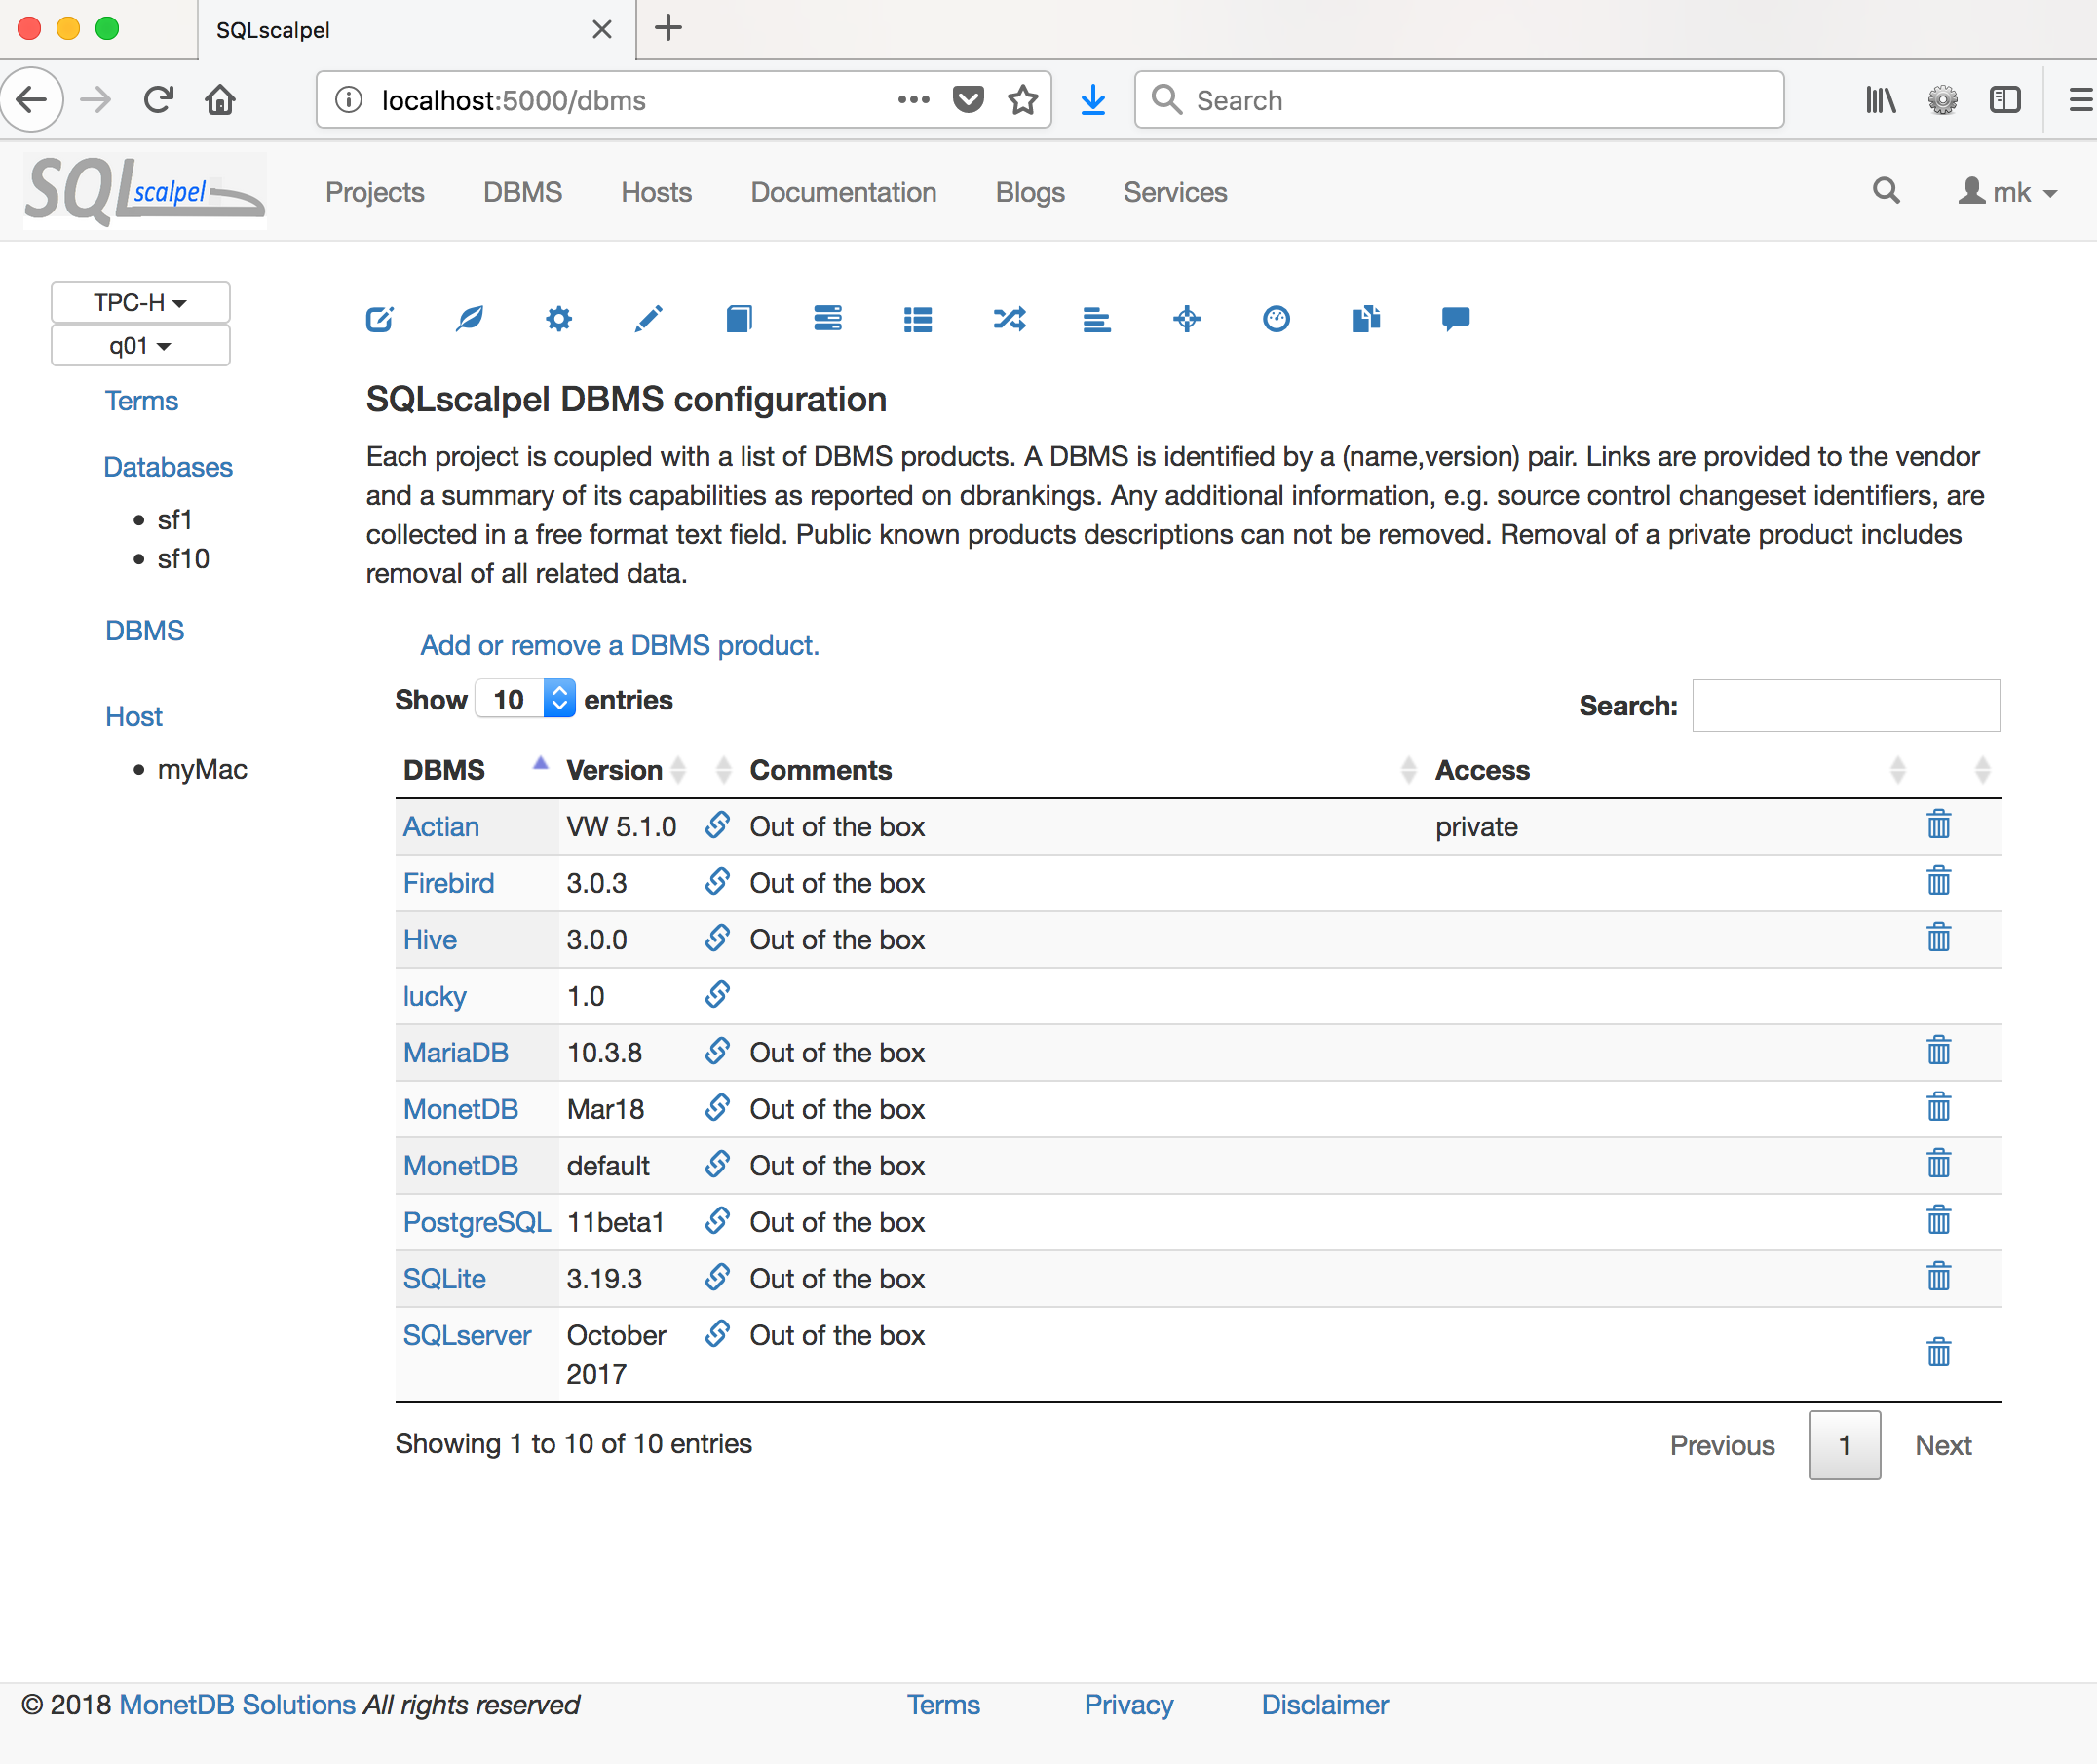
\includegraphics[height=2in,width=3in]{Figures/dbms.png}
%	\caption{DBSMS overview
%		\label{fig:dbms}}
%\end{figure}

%\begin{figure}[t!]
%	\centering
%	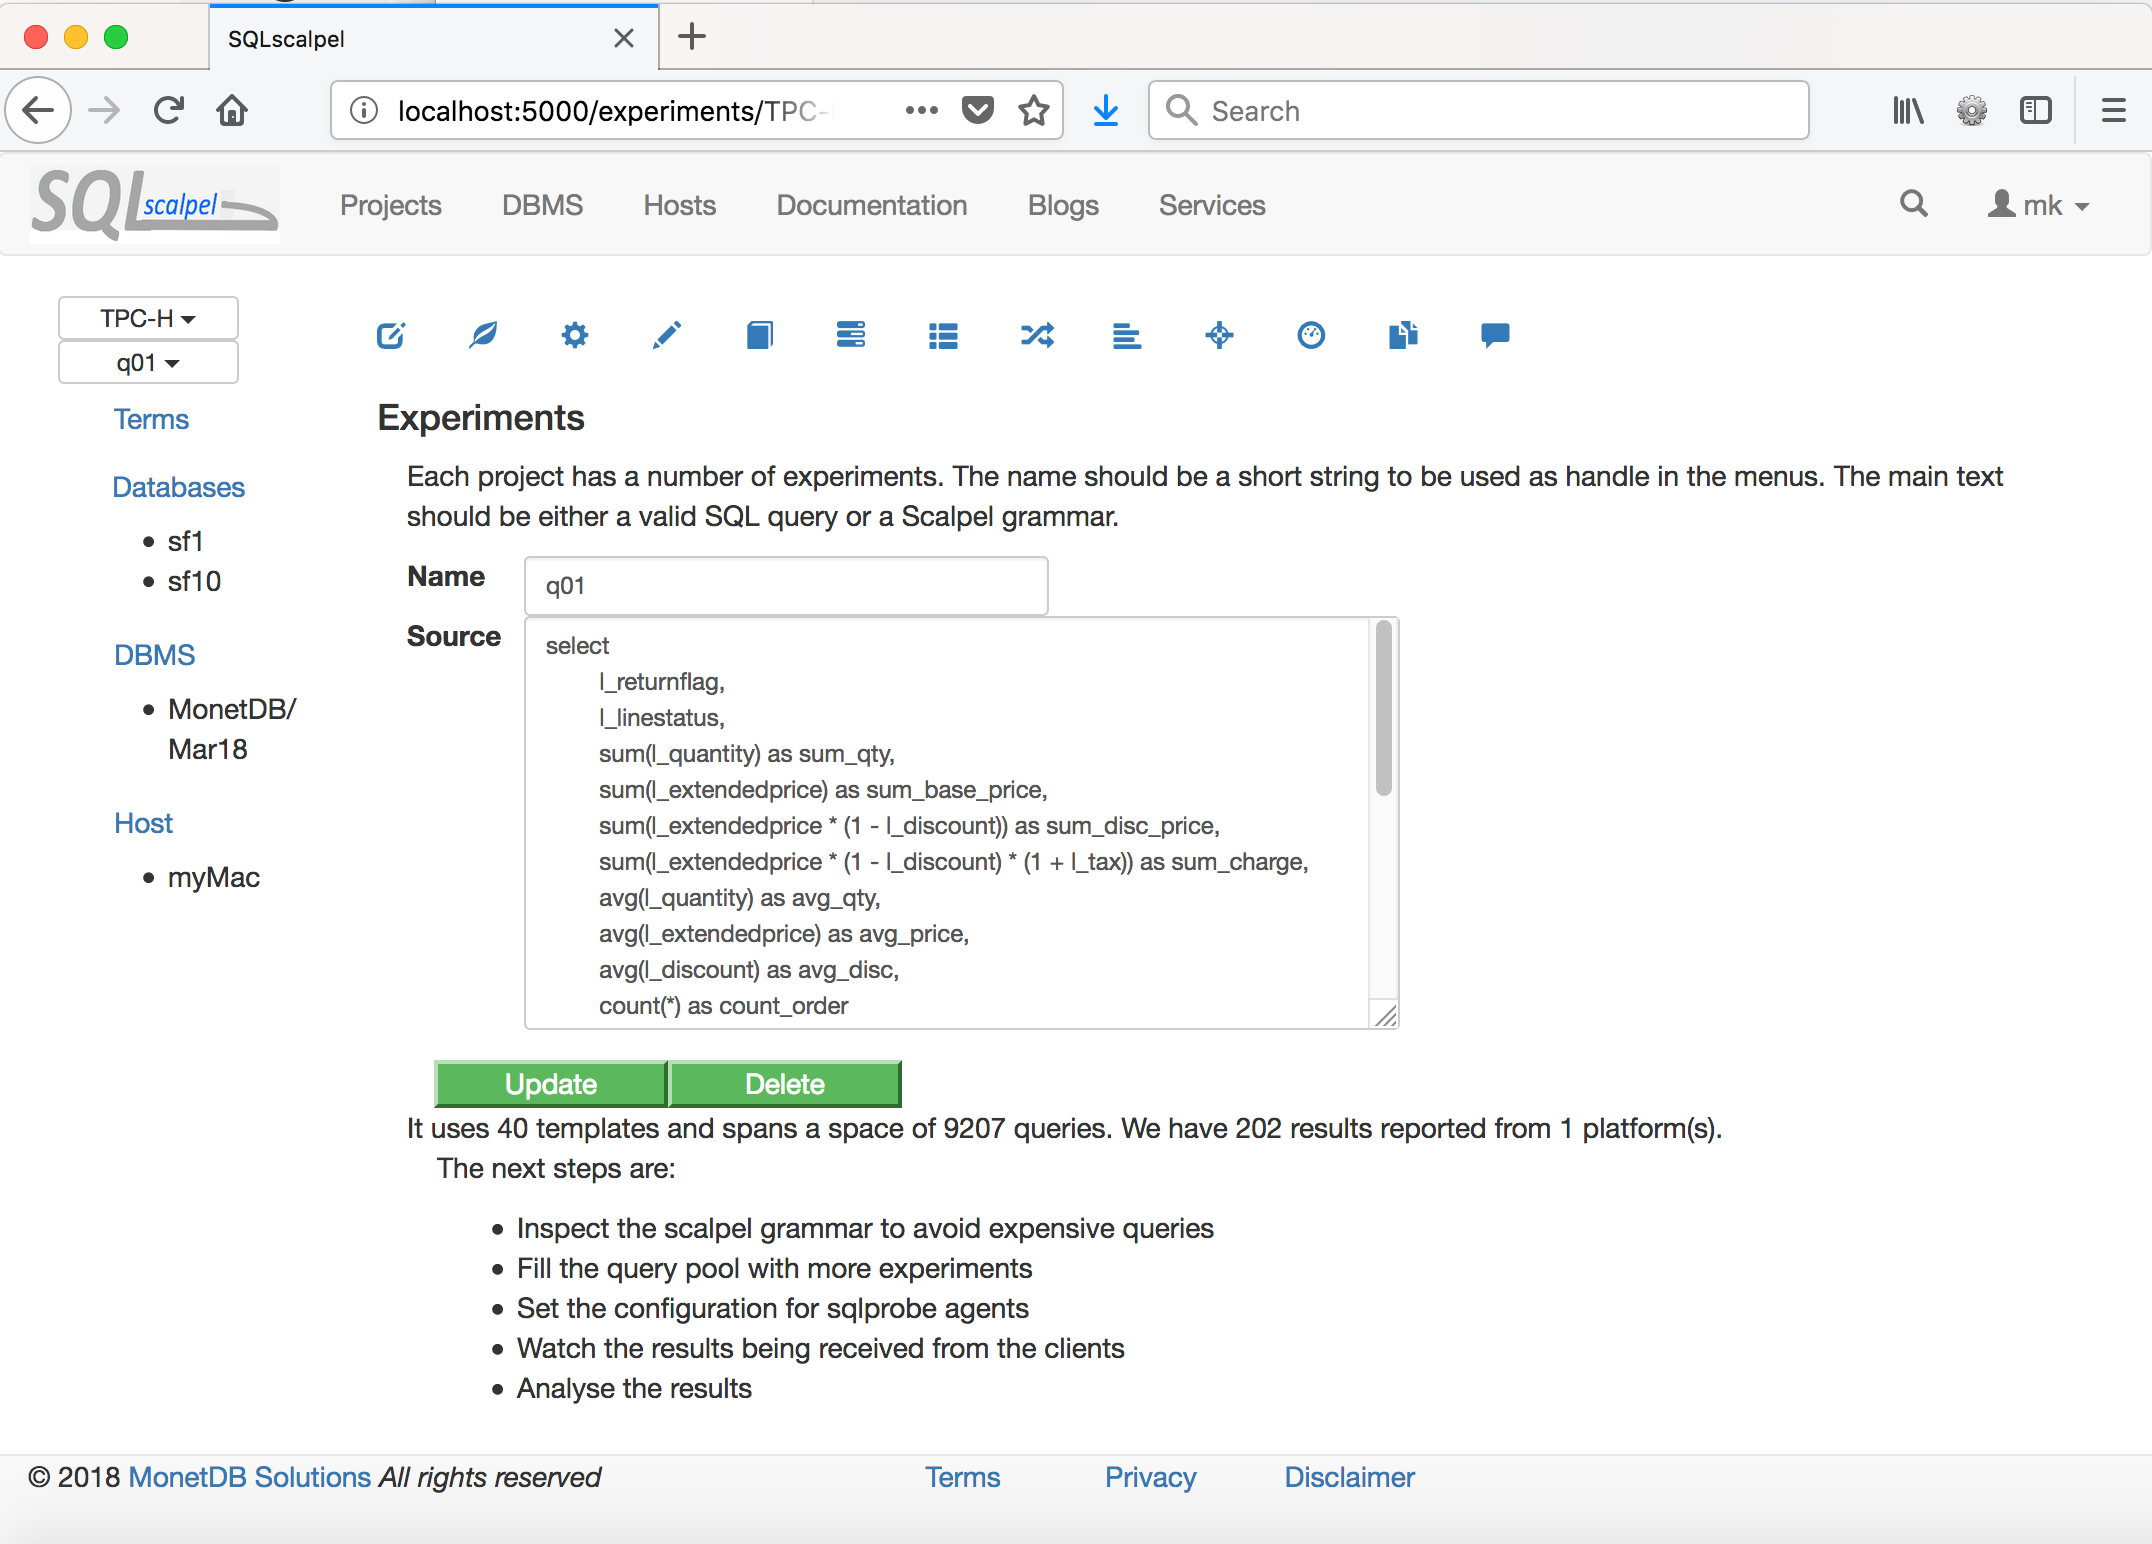
\includegraphics[height=2in,width=3in]{Figures/experiment.png}
%	\caption{Query experiment
%		\label{fig:experiment}}
%\end{figure}

%\begin{figure}[t!]
%\centering
%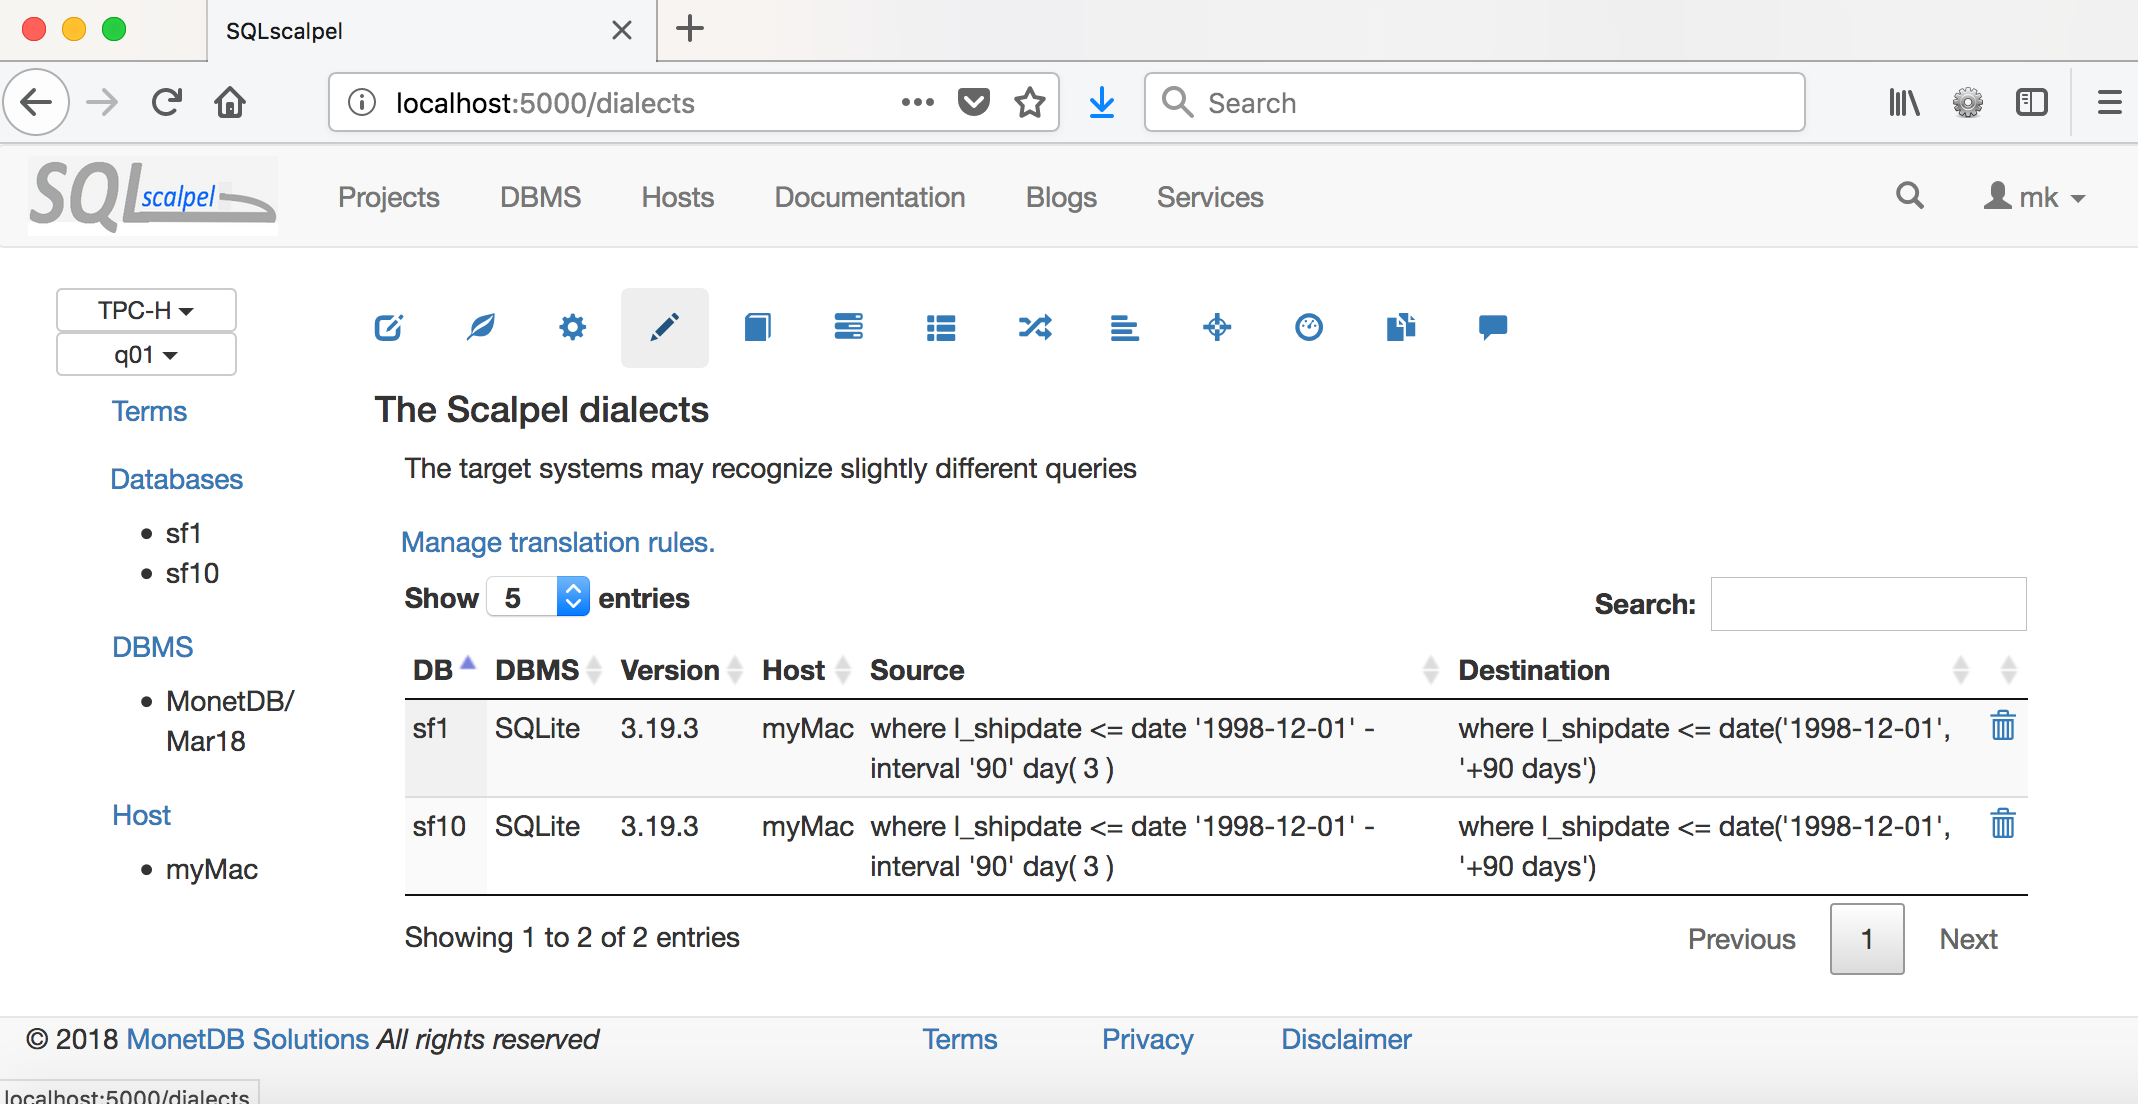
\includegraphics[height=2in,width=3in]{Figures/dialects.png}
%\caption{Query dialects
%	\label{fig:dialects}}
%\end{figure}

\begin{figure*}[t!]
  %pdfcomment{Panos: The figures are really difficult to read and make sense of. If we have the option, maybe we should send an appendix with higher definition screenshots.}
  \centering
  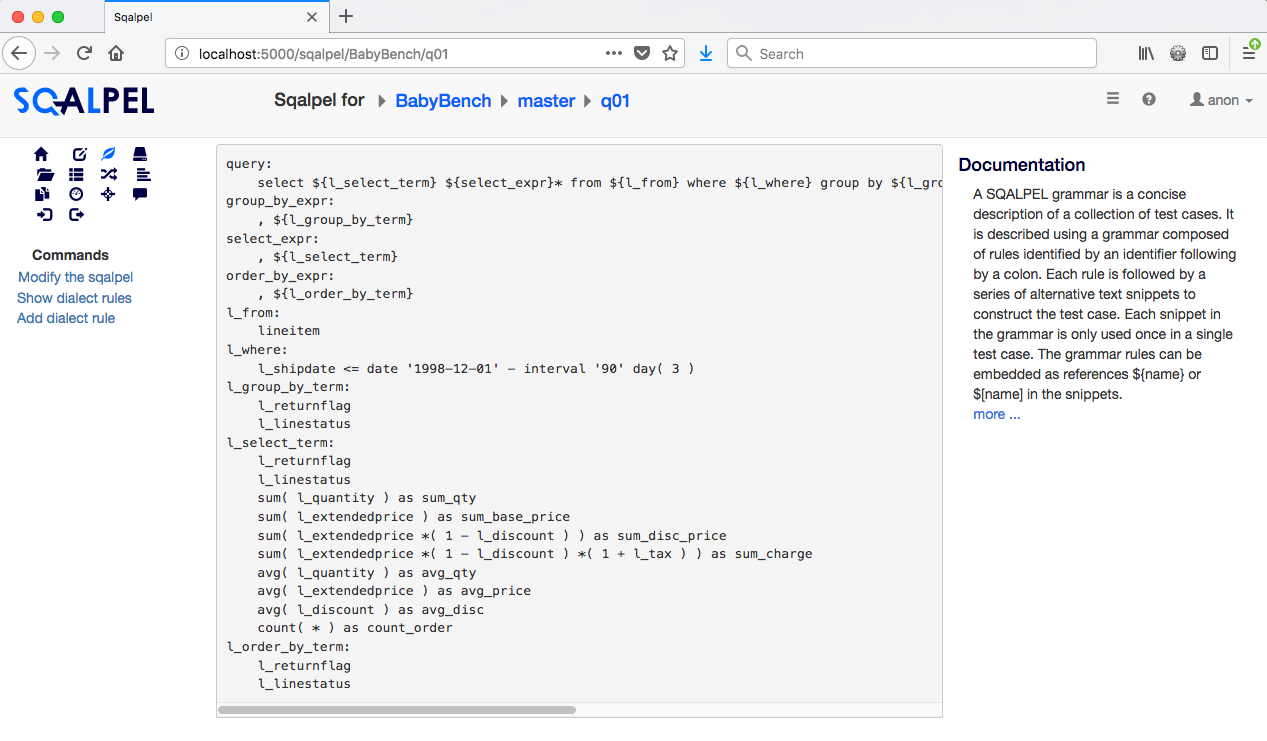
\includegraphics[width=.807\textwidth]{Figures/scalpel2.png}
  \caption{Query {\sc sqalpel}
    \label{fig:sqalpel}}
\end{figure*}


%\begin{figure}[t!]
%\centering
%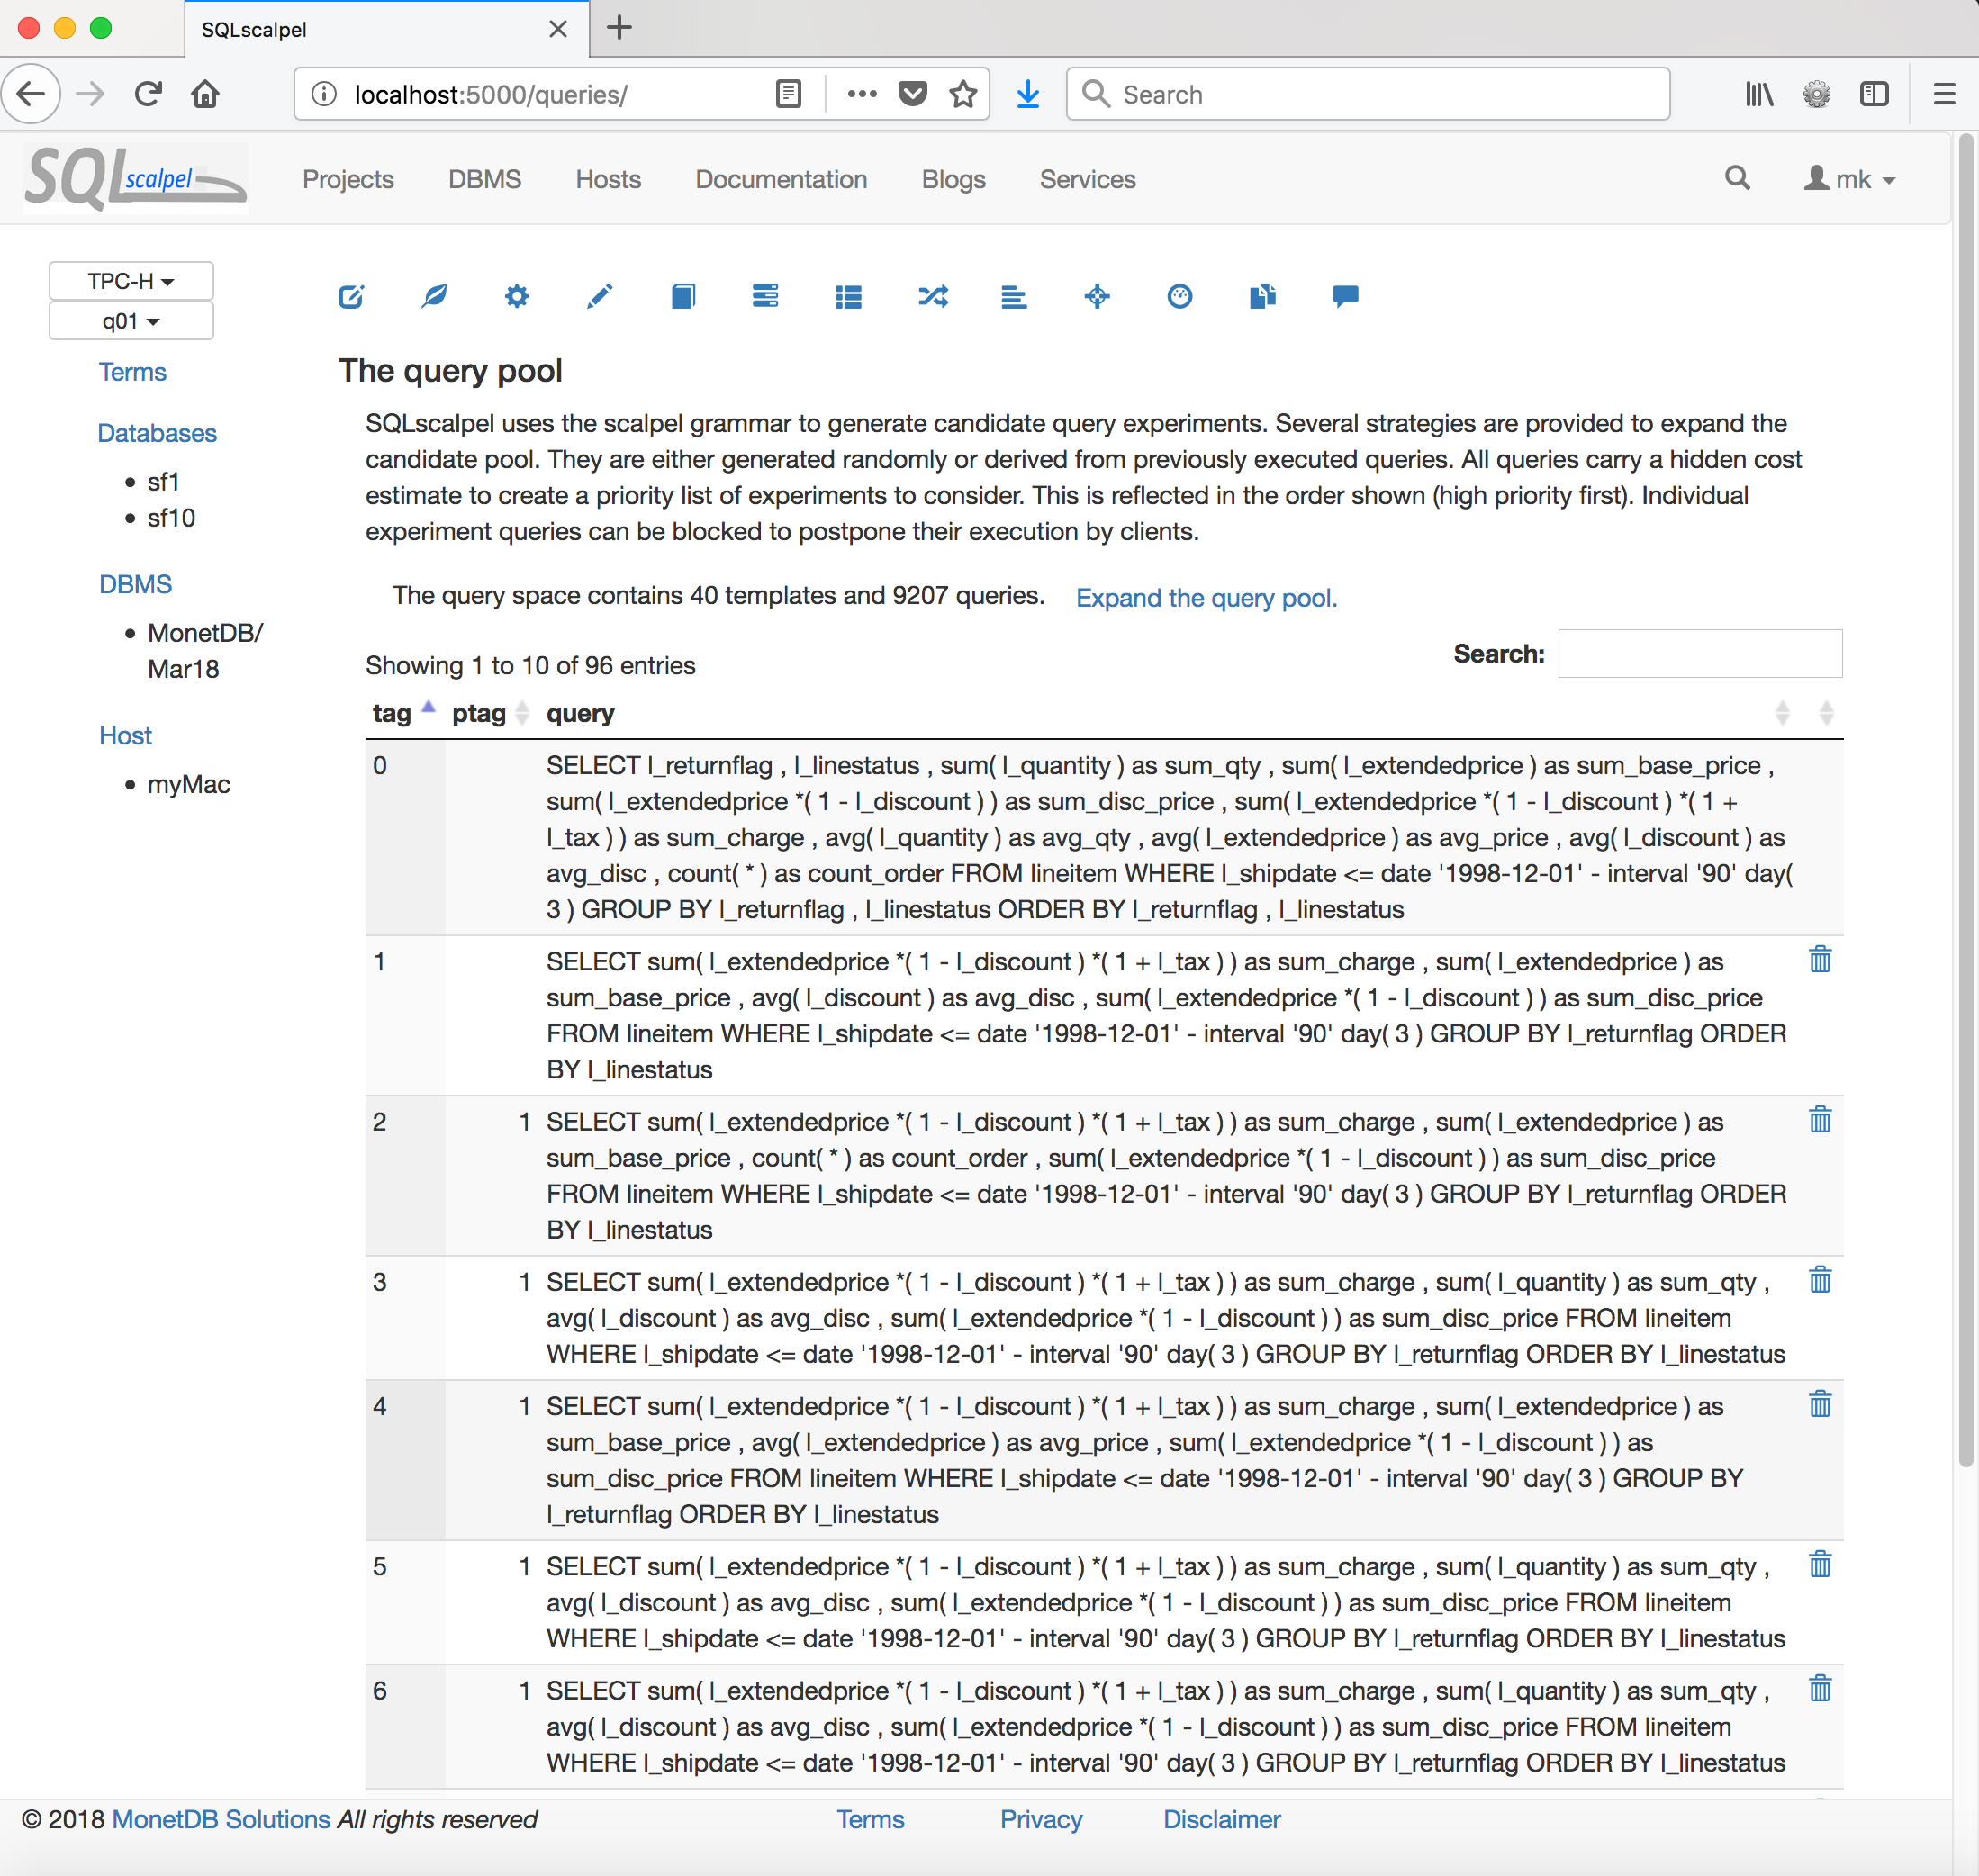
\includegraphics[height=2in,width=3in]{Figures/querypool.png}
%\caption{Query pool
%	\label{fig:querypool}}
%\end{figure}

\begin{figure*}[t!]
\centering
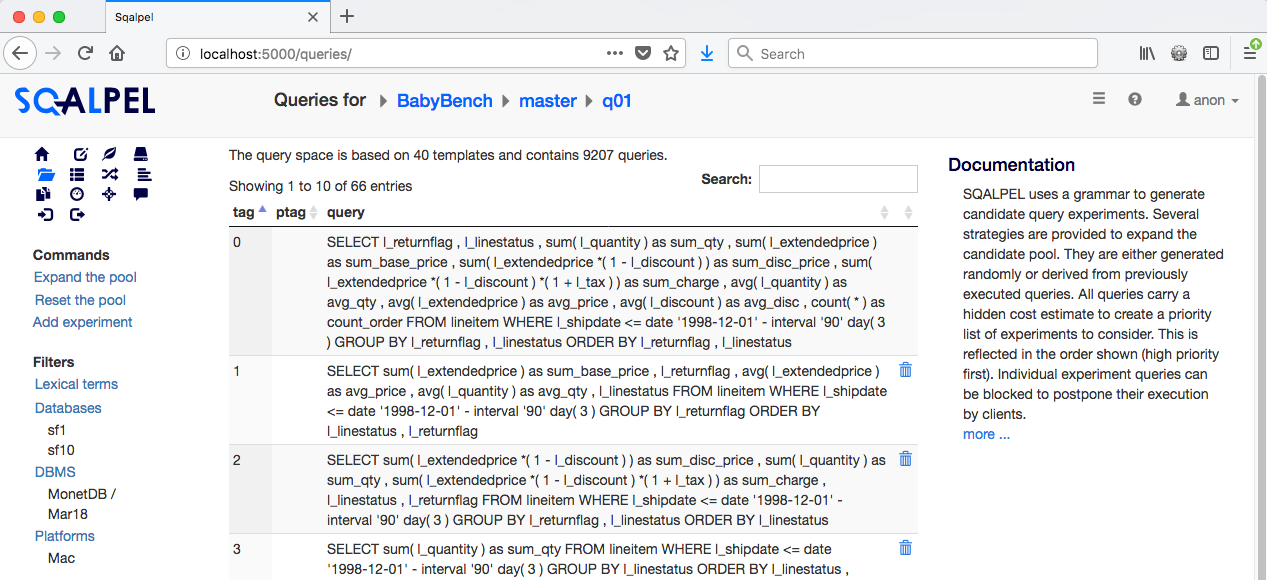
\includegraphics[width=.807\textwidth]{Figures/querypool2.png}
\caption{Query pool
	\label{fig:querypool2}}
\end{figure*}

\begin{figure*}[t!]
\centering
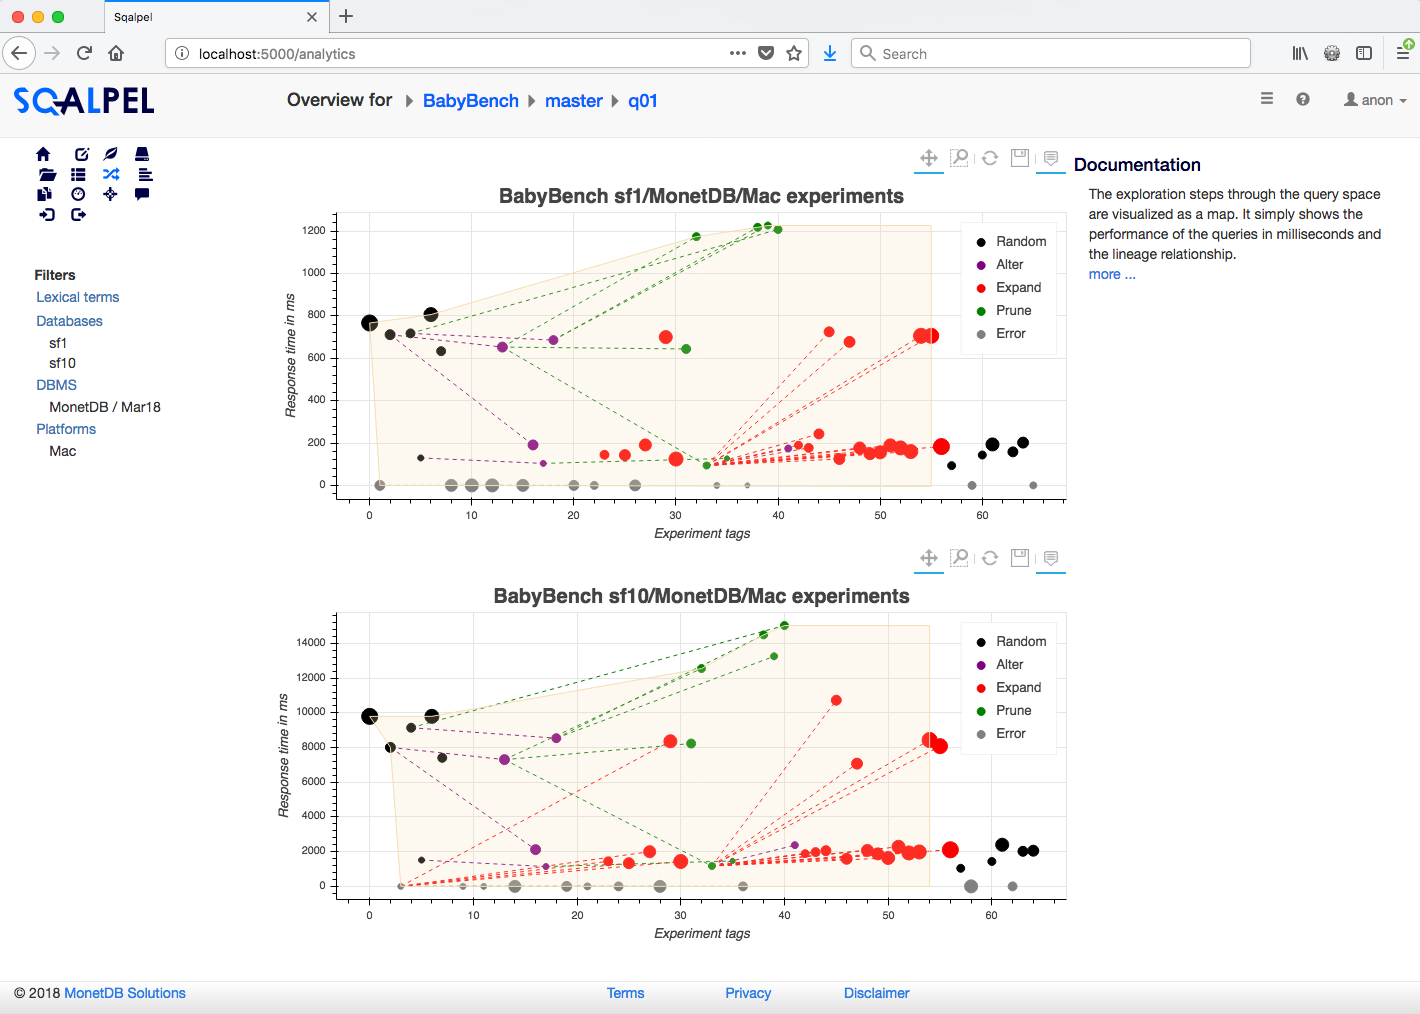
\includegraphics[width=.807\textwidth]{Figures/history2.png}
\caption{Experiment history
	\label{fig:history}}
\end{figure*}

\begin{figure*}[t!]
\centering
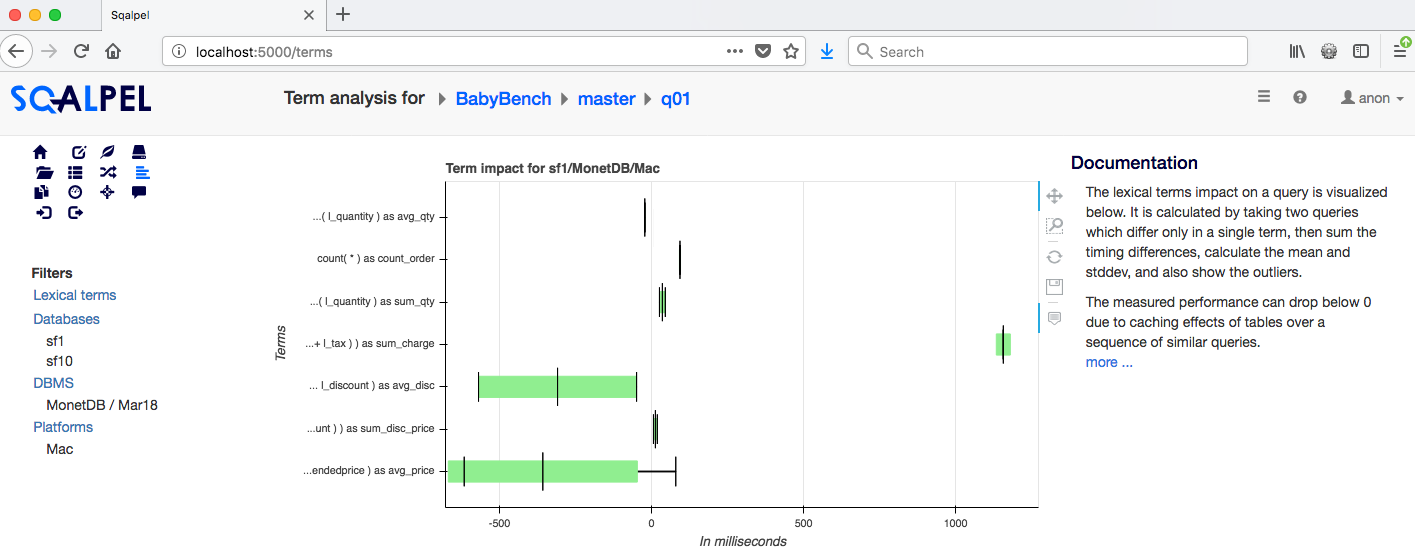
\includegraphics[width=.807\textwidth]{Figures/components2.png}
\caption{Principle components
	\label{fig:components}}
\end{figure*}

%\begin{figure*}[t!]
%\centering
%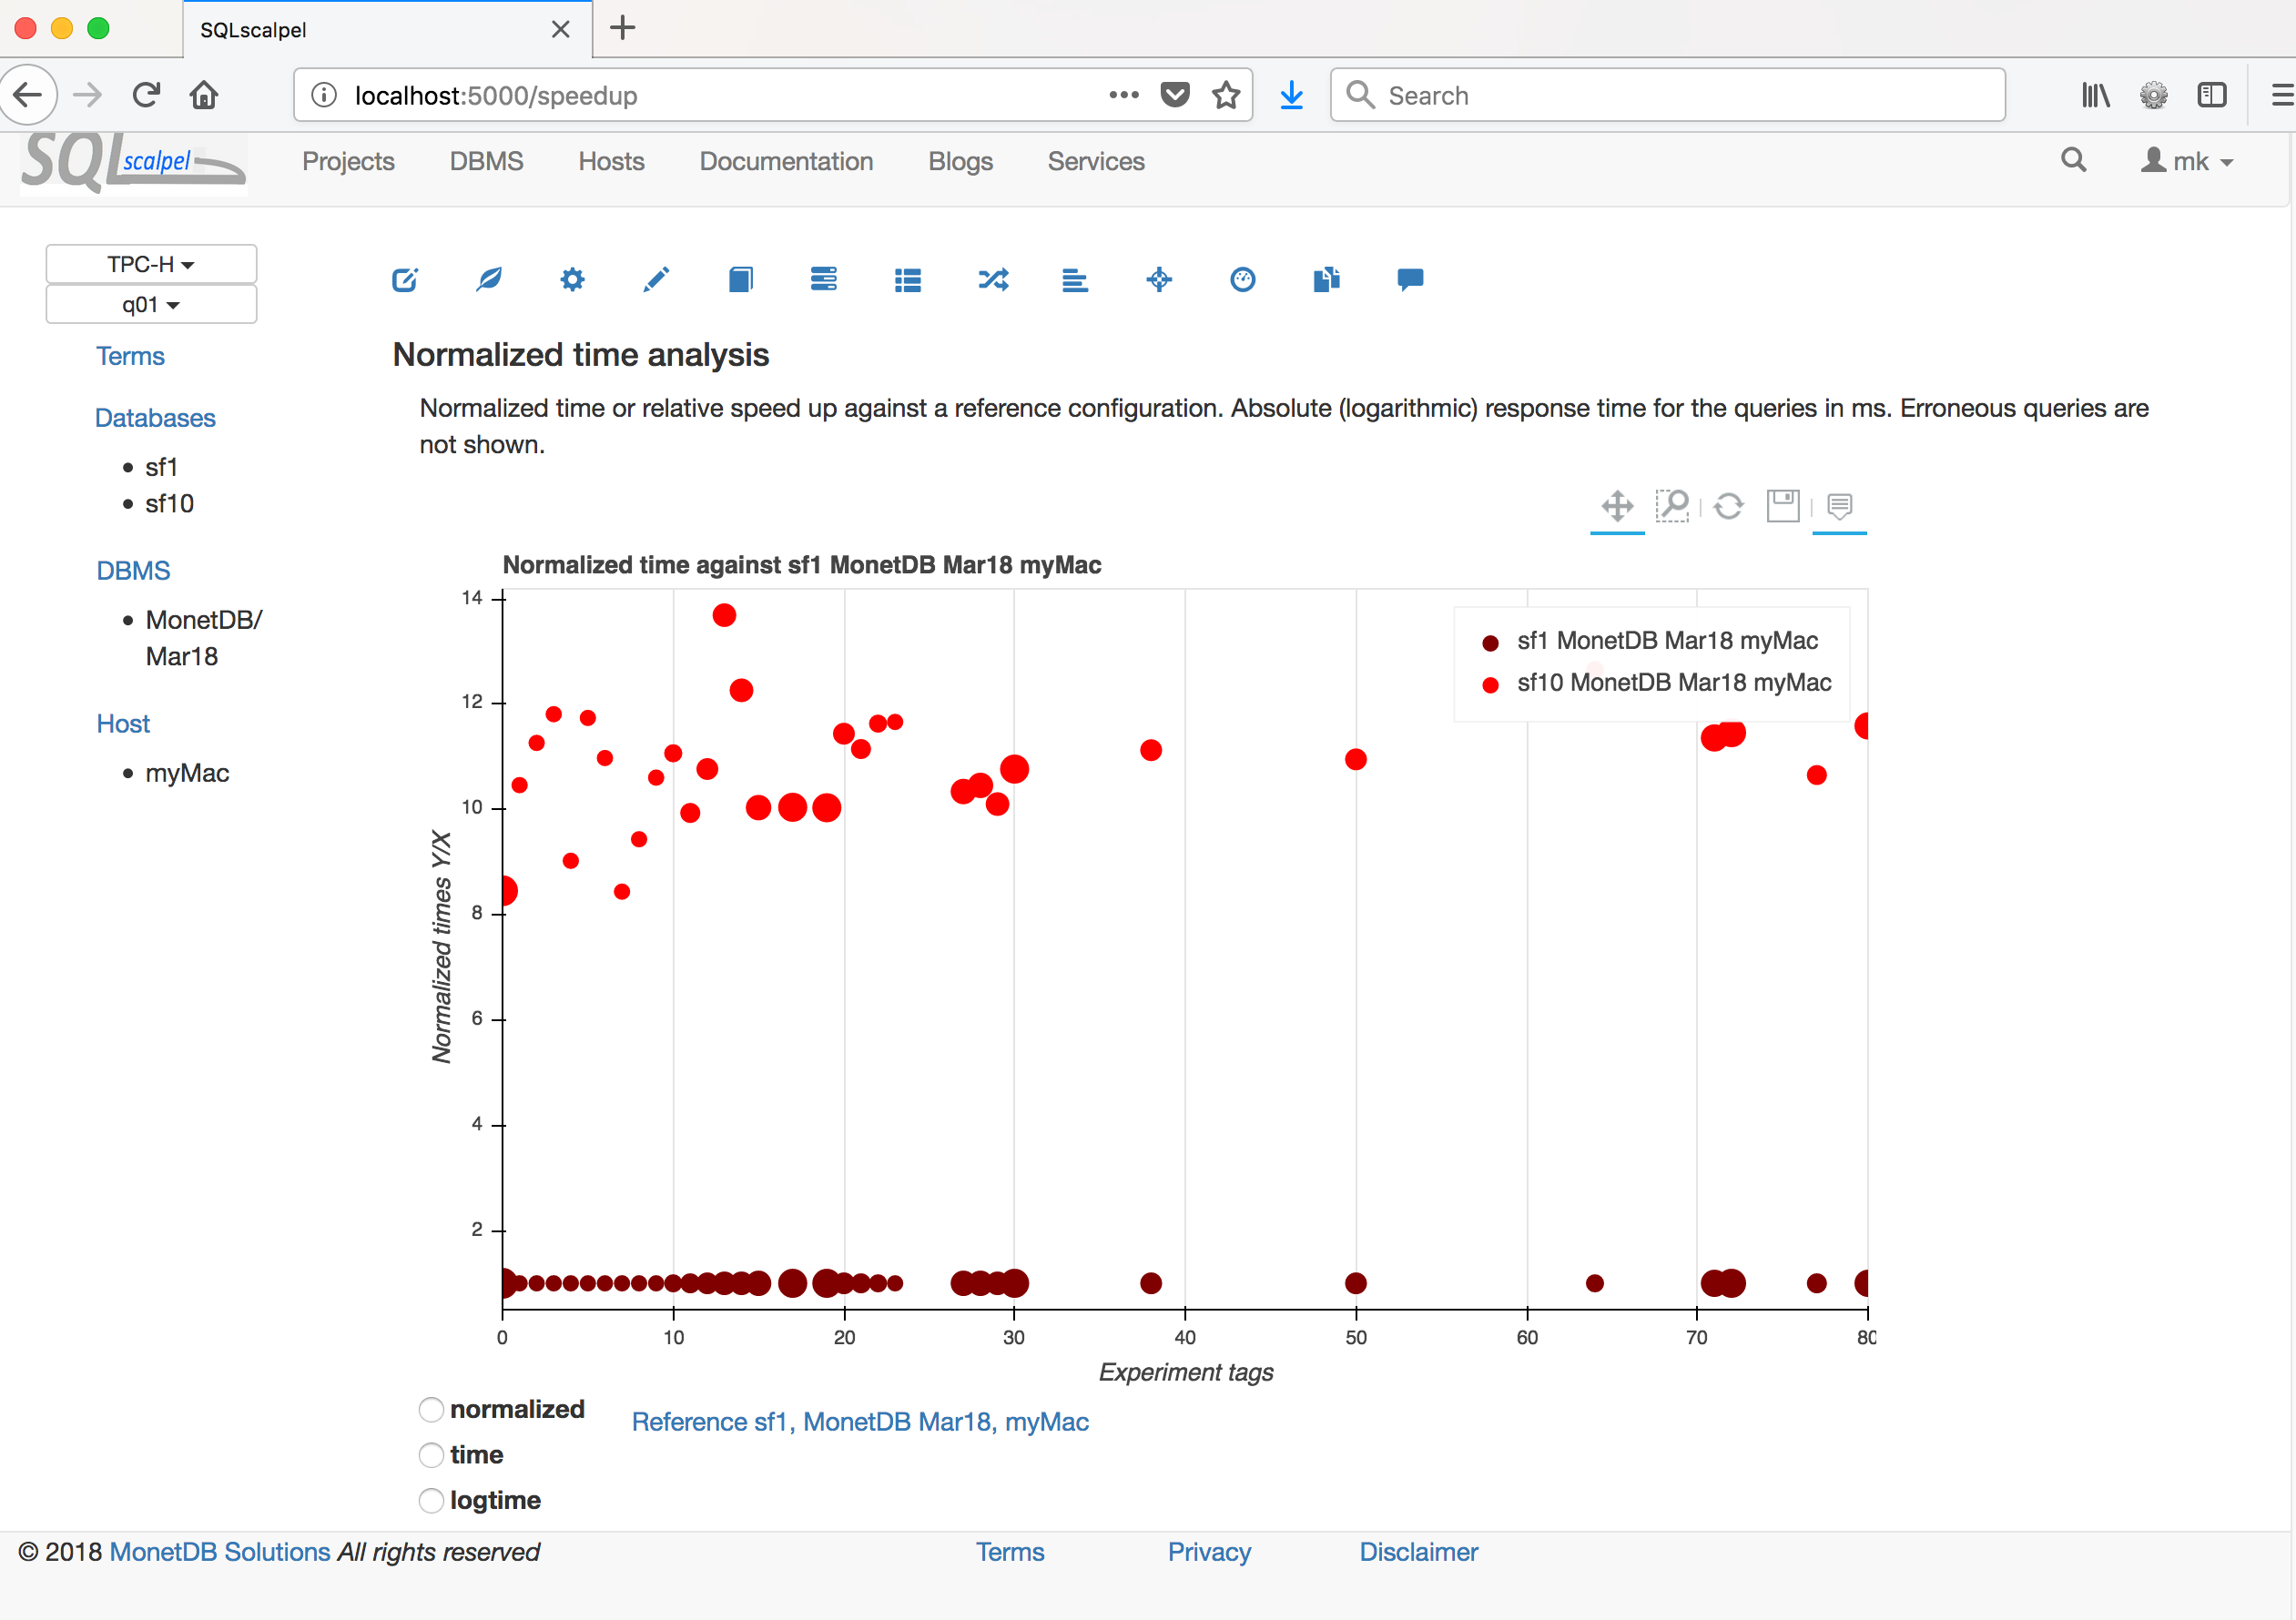
\includegraphics[height=2in,width=3in]{Figures/speedup.png}
%\caption{Query speedup
%	\label{fig:speedup}}
%\end{figure*}

\begin{figure*}[t!]
\centering
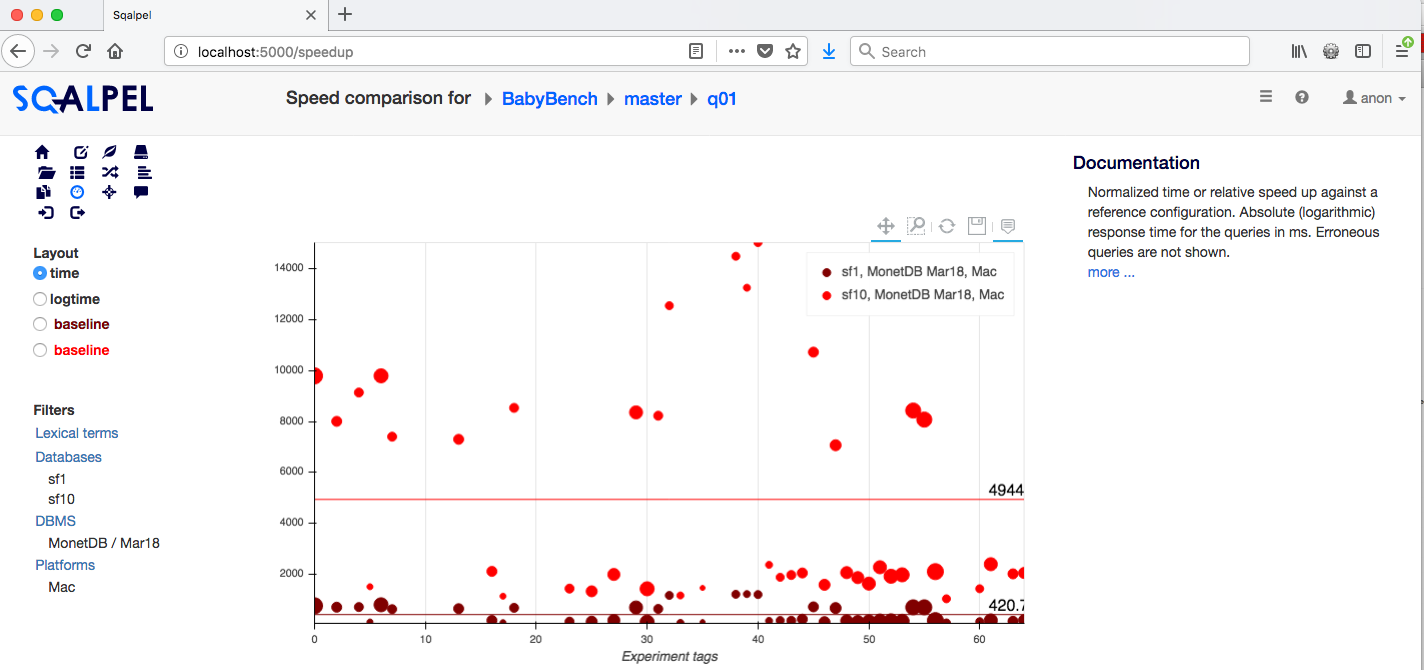
\includegraphics[width=.807\textwidth]{Figures/speedup3.png}
\caption{Query speedup
	\label{fig:speedup2}}
\end{figure*}

\begin{figure*}[t!]
\centering
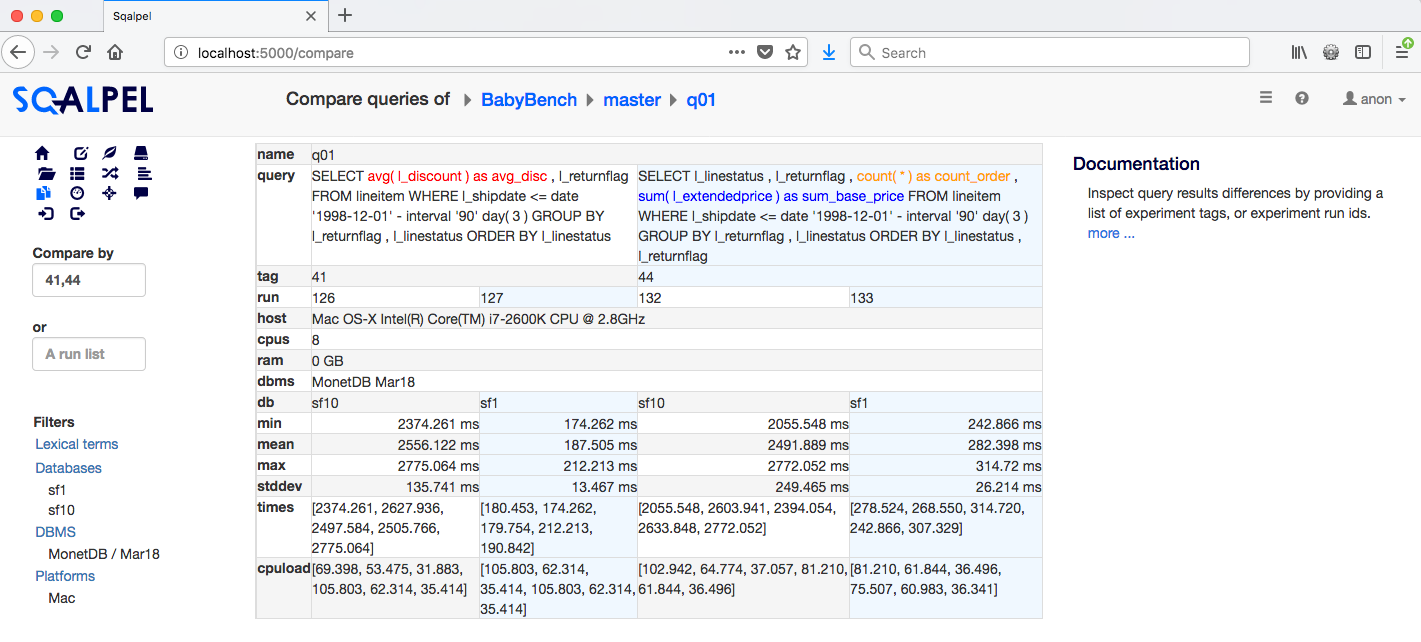
\includegraphics[width=.807\textwidth]{Figures/compare2.png}
\caption{Query differentials
	\label{fig:differential}}
\end{figure*}




%\begin{figure}[t!]
%\centering
%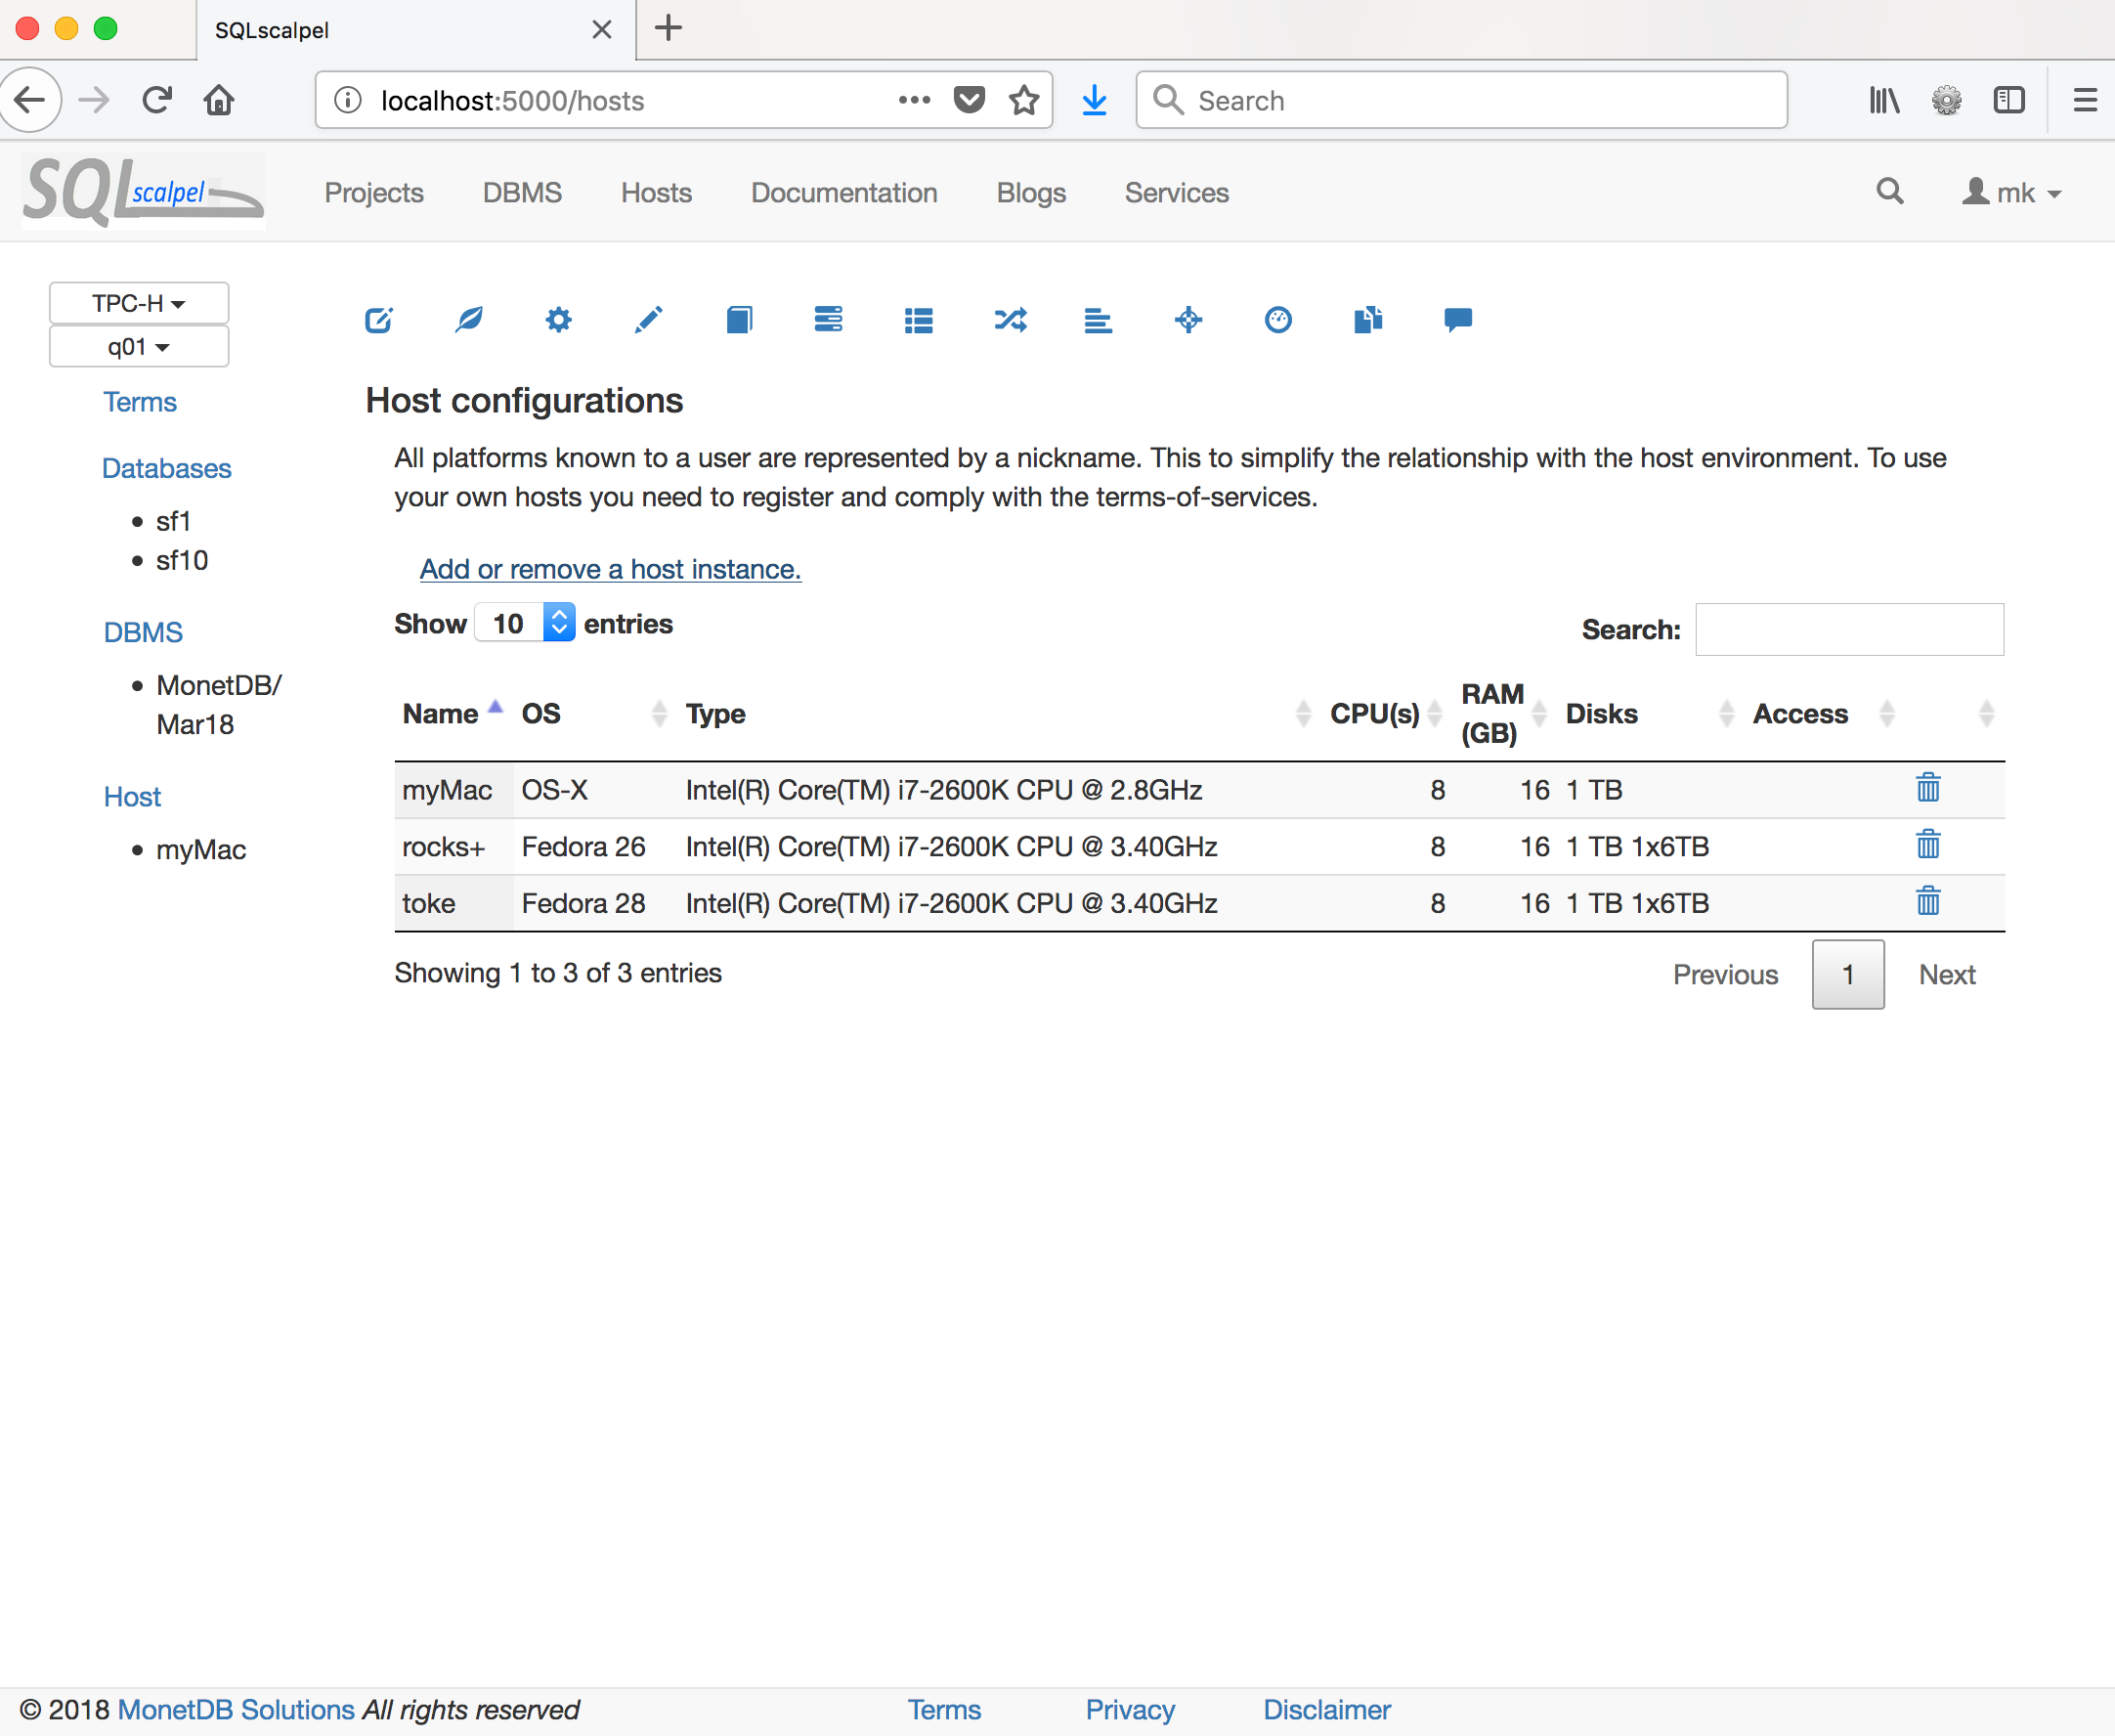
\includegraphics[height=2in,width=3in]{Figures/hosts.png}
%\caption{Hosts
%	\label{fig:hosts}}
%\end{figure}





%The hypothese
%The measurement
%The results and insight

%\subsection{Clickhouse}
%We have been given the opportunity to run the experiments reported by Clickhouse on their original data. The prime reason was to validate ~\footnote{The times for MonetDB relate to an ancient version, beginning of 2013} the reported performance on their website and to understand what queries in their application space caused the huge performance differences. The query set consists of just 43 queries picked randomly by hand from their application setting, i.e.\ web-log analysis.

%To challenge {\sc sqalpel} we simply combined all the queries into one big grammar. It already showed that the benchmark was using only 34 out of 104 columns of their database table. Furthermore, as few as 19 predicate terms where used to filter out records and 16 columns were used to group information.
%The grammar analysis leads to 14K different query templates and the complete space of $> ~ 10 ^{22}$ different queries. If their choice of 43 queries properly represents this space remains to be seen. One observation in deploying it with {\sc sqalpel} showed that there are essentially two outstanding discriminative queries. In a hot database setting, MonetDB performs much better on point-queries, while it performed worst against Clickhouse when confronted by aggregation over a large number of small groups. Given the biased query distribution this results in a non-representative global comparison figure and provided insight on where to improve MonetDB.

%\subsection{The real world}
%Another driving example for {\sc sqalpel} was a problematic customer query. It was a typical BI query, generated by a front-end tool and heavily relying on expanding (inline) views. The result was a single SQL statement of $\sim$2K lines ($\sim$ 110 K characters), which included 68 subqueries, $>100$ (dis/con)junctive terms and much of the SQL functionality, i.e.\ group-by, order-by, case-expressions, window-based aggregates, casting, etc.

%The query complexity is large enough to make it hard for a human to identify what portion is detrimental to the performance. The {\sc sqalpel} parser
%inferred a grammar with 992 rules, 685 literals, and >100K query templates. The
%complexity of this query drove query morphing towards {\em pruning}, where a
%binary dissection of the query into its components should provide the answera.s.a.p.

%% It is the client's responsibility to run a fraction of the queries
%% proposed to shed the dearly needed insight on what component is the culprit in
%% the poor performance observed.

%\subsection{Lessons learned \label{lessons} }
%Using {\sc sqalpel} in all the settings have improved our ability to analyse the performance differences. The main hurdle to take is to design the grammar that can be used to assess system parameters of interest.

\section{Summary and conclusions}\label{Summary and conclusions}
%recap contribution of paper

We provided a progress report on the {\sc sqalpel} project, a sharp
tool in the hands of system architects, DBAs and end-users to
facilitate sharing experimental data.
%It allows them to describe in a concise manner alarge query workspace and rely on guided randomized walks to localize performance pitfalls quickly.
%The workflow is organized such that maximal sharing of experimental results is facilitated.
Saving an enormous amount of energy for the (research) users when
confronted with best-of-breed product selection, or best-of-breed
functionality offerings, or simply measuring progress in science by
standing on the shoulders of giants.



%future extensions
%Possible directions of future research can be inspired by e.g.\ attribute grammars, where each production rule comes with a semantic part to control the generation of the final query. For example, to replace the literal tokens by context dependent values or iterators.

%SQALPEL could have been extended with a full semantic analysis of the SQL query. This however, would invalidate the primary focus. Furthermore, checking for invalid queries is a cheap operation. Morphing an erroneous query into a valid one also remains possible.

%Although {\sc sqalpel} has been initially designed for database query performance analysis, its generality permits any other system comparison to be undertaken as well. Running queries from a search space can readily be replaced by running parameterized scripts to study e.g.\ database loading, database update workloads, messaging systems, compilers, HPC applications, and user interaction scenarios.


\subsection*{Acknowledgments} This research has received funding from the European Union's Horizon 2020 research and innovation programme under Grant Agreement no.~732366 (ACTiCLOUD).

{
%\small	% see makePDF.sh
\bibliography{refs}
\bibliographystyle{abbrv}
}
%\printindex
\end{document}
